\documentclass[a4paper, twoside]{report}

%% Language and font encodings
\usepackage[english]{babel}
\usepackage[utf8x]{inputenc}
\usepackage[T1]{fontenc}

%% Sets page size and margins
\usepackage[a4paper,top=2cm,bottom=2.5cm,left=2cm,right=2cm,marginparwidth=1cm]{geometry}

%% Useful packages
\usepackage{amsmath}
\usepackage{graphicx}
\usepackage{subcaption}
\usepackage{listings}
\usepackage{color}
\lstset{basicstyle=\small\ttfamily,
    keywordstyle=\color{purple}}
\usepackage{tikz}
\usepackage[percent]{overpic}
\usepackage[colorinlistoftodos]{todonotes}
\usepackage[colorlinks=true, allcolors=blue]{hyperref}

\title{Building an Efficient DBMS by Generating OpenCL Code from Voodoo Vector Algebra}
\author{Alexander Clarke \\ Qiang Feng \\ Mayeul Fournial \\ Pranav Kalidindi \\ Jordan Spooner \\ Laurence Squires}
% Update supervisor and other title stuff in title/title.tex

%% Our own style changes
\setlength{\parindent}{0pt}
\setlength{\parskip}{\medskipamount}
\usepackage{tgpagella}

\begin{document}
\begin{titlepage}

\newcommand{\HRule}{\rule{\linewidth}{0.5mm}} % Defines a new command for the horizontal lines, change thickness here

%----------------------------------------------------------------------------------------
%	LOGO SECTION
%----------------------------------------------------------------------------------------


\includegraphics[width=8cm]{title/logo.png}\\[1cm] % Include a department/university logo - this will require the graphicx package
 
%----------------------------------------------------------------------------------------

\center % Center everything on the page

%----------------------------------------------------------------------------------------
%	HEADING SECTIONS
%----------------------------------------------------------------------------------------

\textsc{\LARGE Software Engineering Group Project}\\[1.5cm] % Name of your university/college
\textsc{\Large Imperial College London}\\[0.5cm] % Major heading such as course name
\textsc{\large Department of Computing}\\[0.5cm] % Minor heading such as course title

%----------------------------------------------------------------------------------------
%	TITLE SECTION
%----------------------------------------------------------------------------------------
\makeatletter
\HRule \\[0.4cm]
{ \huge \bfseries \@title}\\[0.4cm] % Title of your document
\HRule \\[1.5cm]
 
%----------------------------------------------------------------------------------------
%	AUTHOR SECTION
%----------------------------------------------------------------------------------------

\begin{minipage}{0.4\textwidth}
\begin{flushleft} \large
\emph{Authors:}\\
\@author % Your name
\end{flushleft}
\end{minipage}
~
\begin{minipage}{0.4\textwidth}
\begin{flushright} \large
\emph{Supervisor:} \\
Dr. Holger Pirk \\[1.2em] % Supervisor's Name
\end{flushright}
\end{minipage}\\[2cm]
\makeatother

% If you don't want a supervisor, uncomment the two lines below and remove the section above
%\Large \emph{Author:}\\
%John \textsc{Smith}\\[3cm] % Your name

%----------------------------------------------------------------------------------------
%	DATE SECTION
%----------------------------------------------------------------------------------------

{\large \today}\\[2cm] % Date, change the \today to a set date if you want to be precise

\vfill % Fill the rest of the page with whitespace

\end{titlepage}

\renewcommand{\abstractname}{Acknowledgements}
\begin{abstract}
We would like to thank Holger Pirk for his continuous guidance and support. We would also like to thank Robert Chatley for the invaluable advice from each of our software engineering consultations.
\end{abstract}

\tableofcontents

\chapter{Executive Summary}

Elevator pitch...

\chapter{Introduction}

\section{Background}

Most of today's popular relational databases use a \emph{Volcano}-style iterator model \cite{Graefe:1994:VEP:627290.627558} for query processing. In this processing model, each operator (say, a projection, selection, join, etc.) produces a stream of tuples. The output stream of another operator is consumed using a simple interface, consisting only of the functions \texttt{open()}, \texttt{next()} and \texttt{close()}. Figure \ref{fig:volcano-processing} demonstrates this approach.

Whilst these databases benefit from a clean and flexible design which maximises maintainability and developer productivity, the Volcano-style processing model makes excessive use of function calls. For example, consider alone the \texttt{next()} call, which must be made for every tuple in the input, each intermediate result, and the final result. As main memory has grown, it is now often the CPU which determines query processing performance, and these function calls lead to frequent instruction mispredictions, and by extension control hazards, requiring CPU stalls which significantly degrade performance.

Database systems such as \emph{MonetDB} \cite{Boncz:2008:BMW:1409360.1409380} pioneered a bulk-processing approach, shown in figure \ref{fig:bulk-processing}, which, instead of considering one tuple at a time, considers entire columns at a time. The benefit of this approach is that the cost of calling the next operator is amortised over the number of tuples. However, it also introduces a new cost: intermediate results must now be materialised. Whilst the iterator-model can pipeline most operators (that is, the output of one operator can be passed directly to the input of the next), this is no longer possible with the bulk-processing model, which must make all resulting tuples accessible to the next operator to process at once. This often results in memory bandwidth constraining performance.

In an attempt to solve this, a new query engine, \emph{X100} \cite{DBLP:conf/cidr/BonczZN05} (which later evolved into VectorWise), was built for MonetDB, which processes smaller (say 1000-value) vectors, which form chunks of columns. These vectors can fit in the CPU cache, and can be pipelined to avoid expensive materialisation.

More recently, the \emph{HyPer} in-memory database system \cite{Neumann:2011:ECE:2002938.2002940} was shown to significantly outperform MonetDB and VectorWise in most cases, by using LLVM to compile queries into machine code with better locality and a more predictable branch layout. In this approach, chains of operators which can be pipelined (i.e. chains that do not require materialisation) are identified, and each of these fragments is compiled separately into machine code, as shown in figure \ref{fig:code-generation}. This reverses the direction of data-flow control: instead of each operator asking its input for tuples, each fragment of code processes the data and makes it available to the next fragment. Operators within each fragment leave tuples inside the CPU registers and so are extremely cheap, whilst pipeline-breaking operators (at the edge of fragments) would have required materialisation anyway, so there is no significant performance implication for them.

\begin{figure}
\centering
\begin{subfigure}[b]{0.49\textwidth}
    \centering
    \begin{tabular}{|c|}
    \hline
    \begin{lstlisting}[language=SQL]
SELECT
  "c_nationkey",
  COUNT("c_custkey")
    AS "customers_in_debt"
FROM
  "customer"
  JOIN "nation"
    ON "c_nationkey" = "n_nationkey"
WHERE
  "c_acctbal" < 0 
GROUP BY
  "c_nationkey"
    \end{lstlisting} \\
    \hline
    \end{tabular}
    \caption{A simple SQL query}
    \label{fig:simple-query}
\end{subfigure}
\begin{subfigure}[b]{0.49\textwidth}
    \centering
    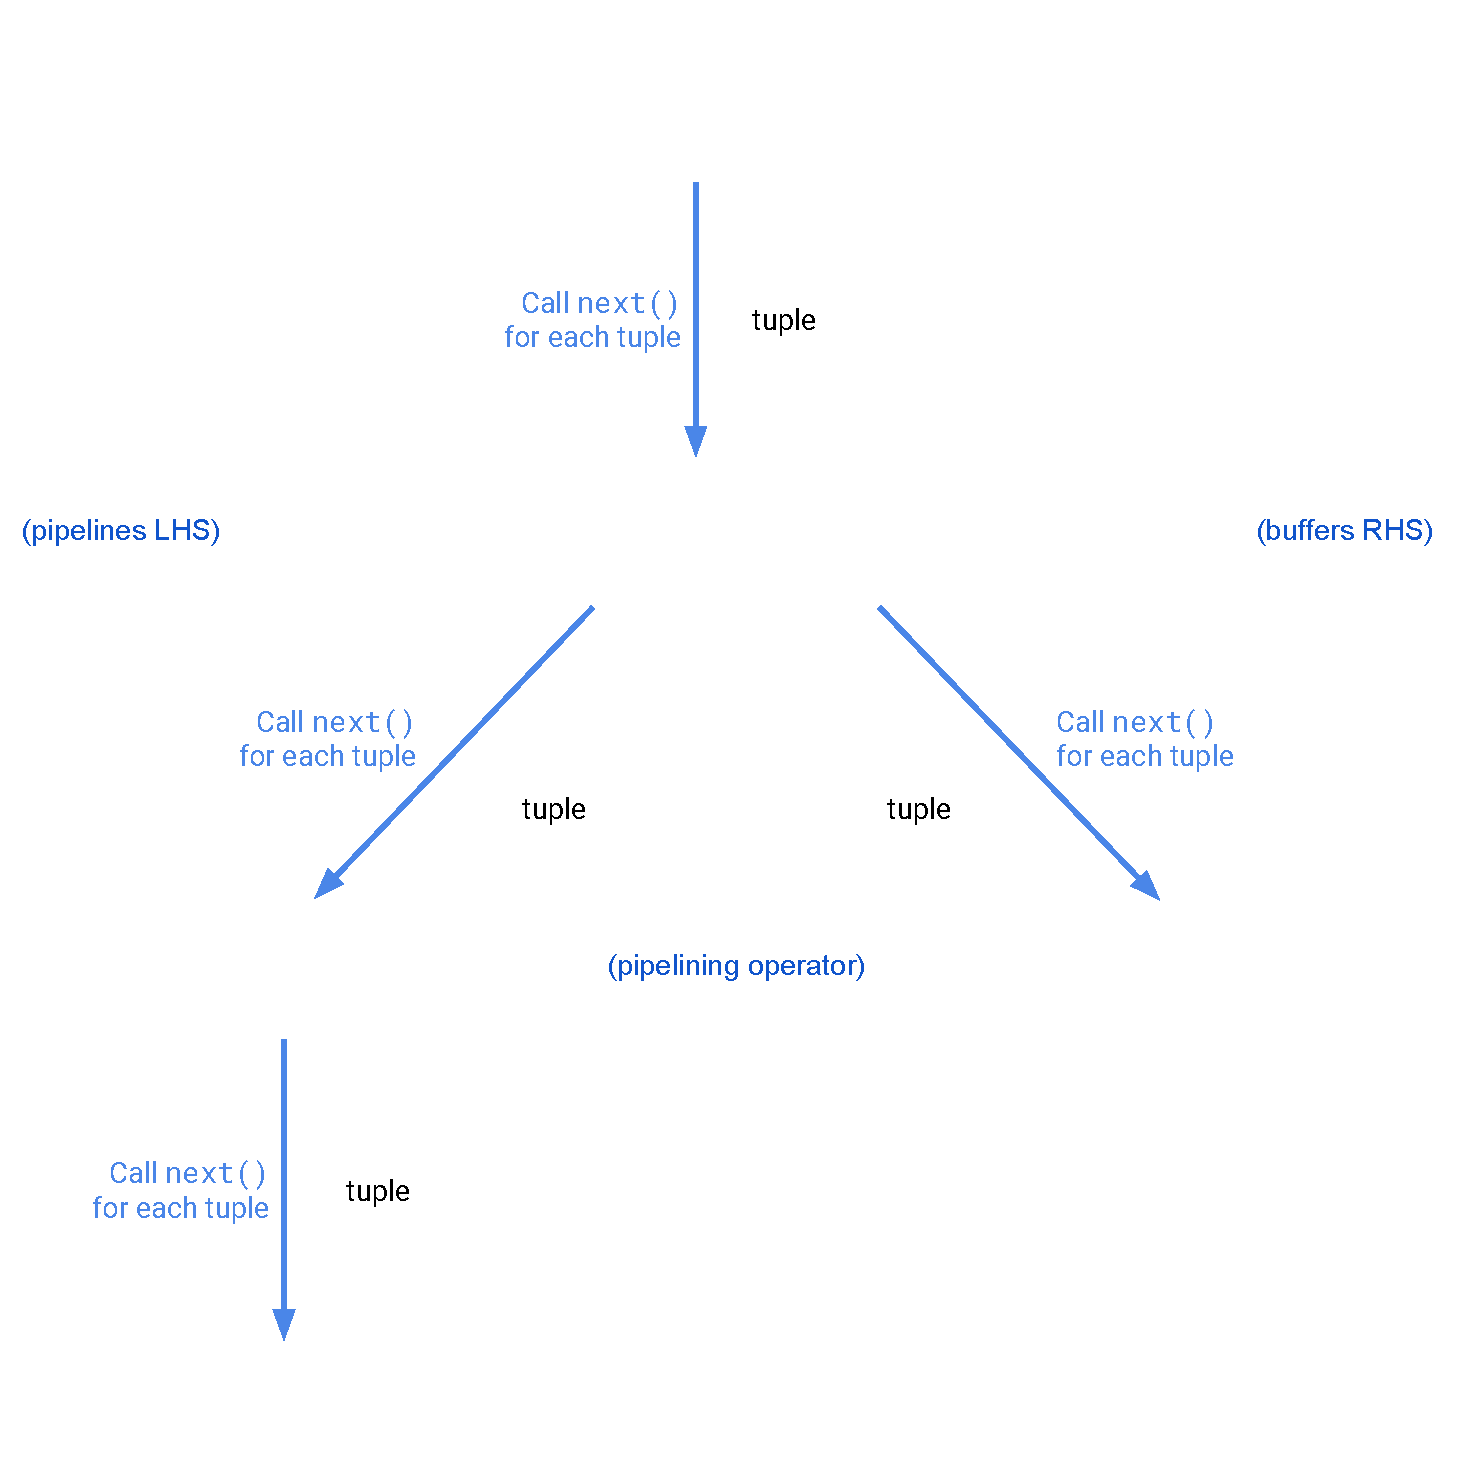
\includegraphics[width=0.9\linewidth]{introduction/volcano.pdf}
    \caption{Evaluating \ref{fig:simple-query} using Volcano processing}
    \label{fig:volcano-processing}
\end{subfigure}
\\[5ex]
\begin{subfigure}[b]{0.49\textwidth}
    \centering
    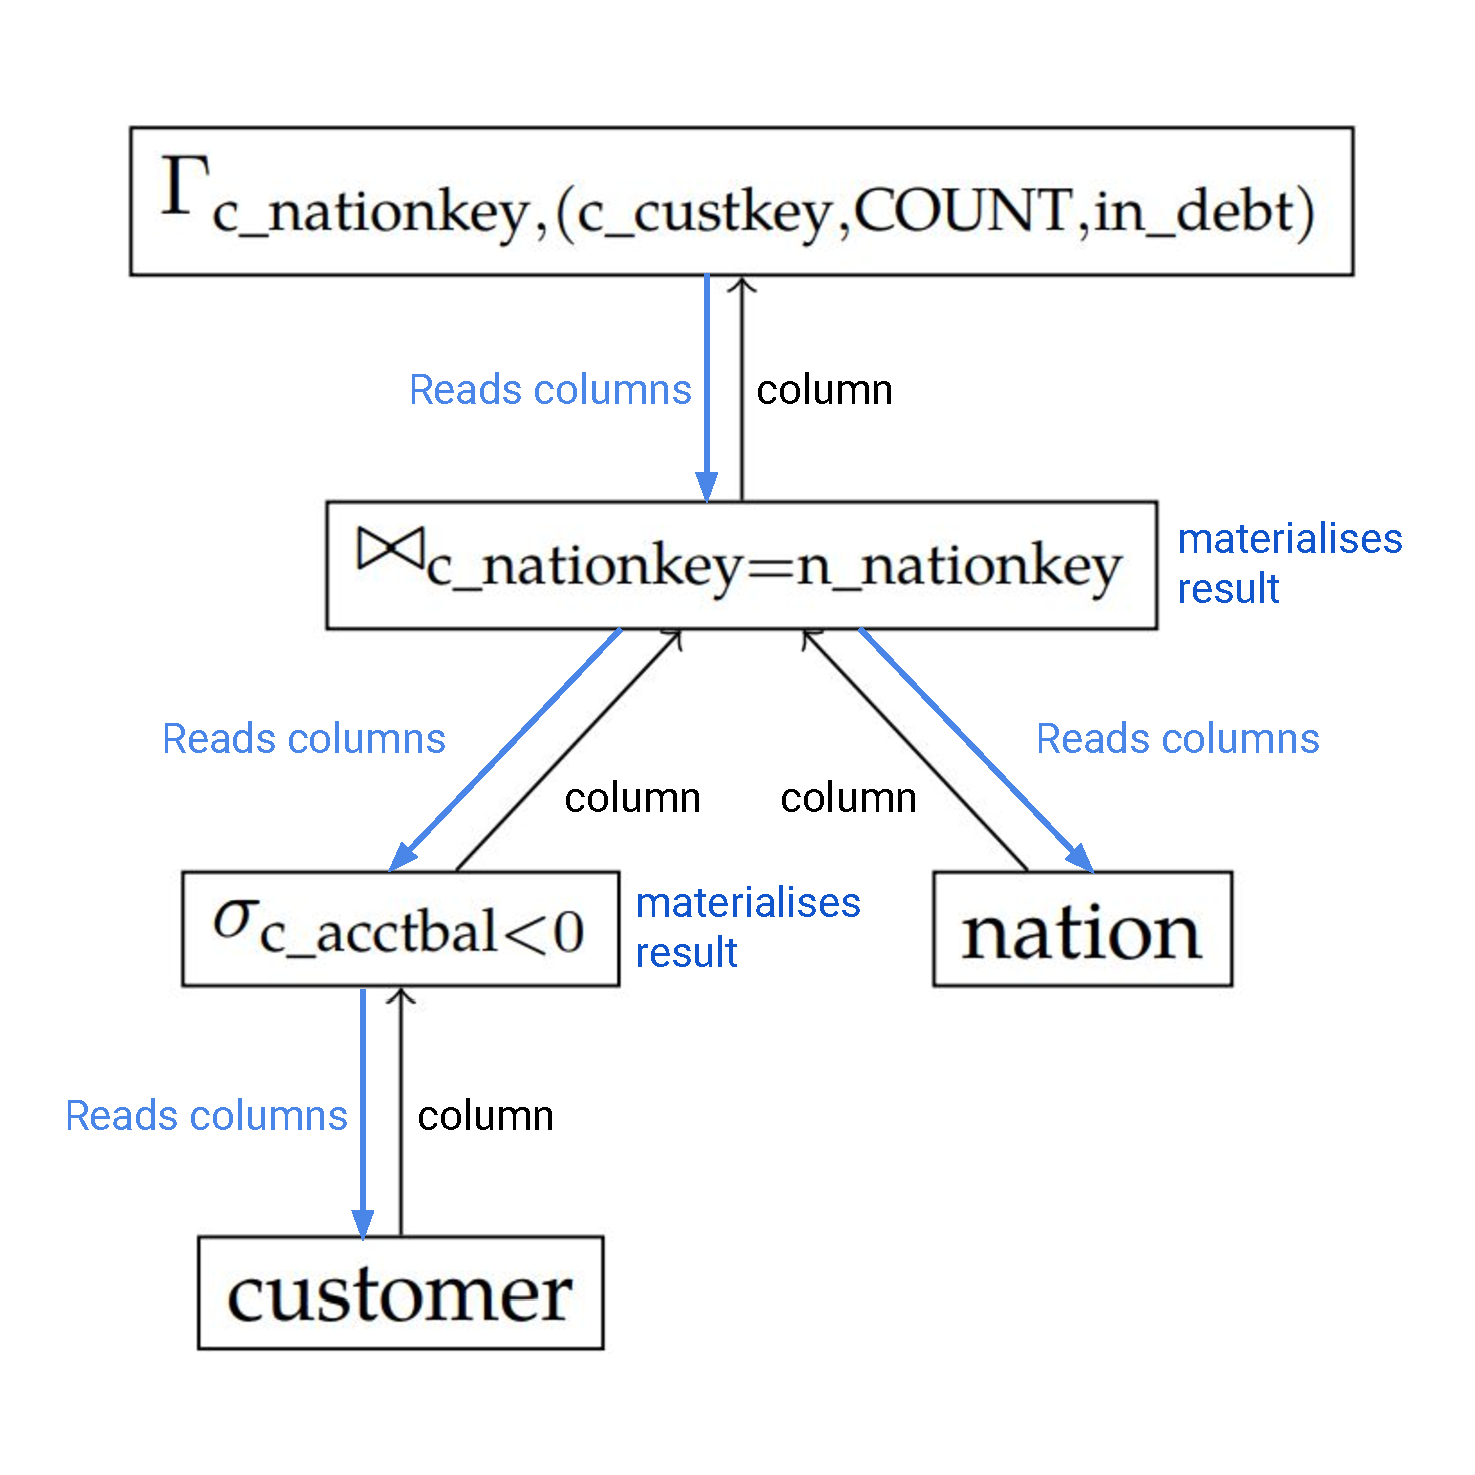
\includegraphics[width=0.9\linewidth]{introduction/bulk.pdf}
    \caption{Evaluating \ref{fig:simple-query} using bulk processing}
    \label{fig:bulk-processing}
\end{subfigure}
\begin{subfigure}[b]{0.49\textwidth}
    \centering
    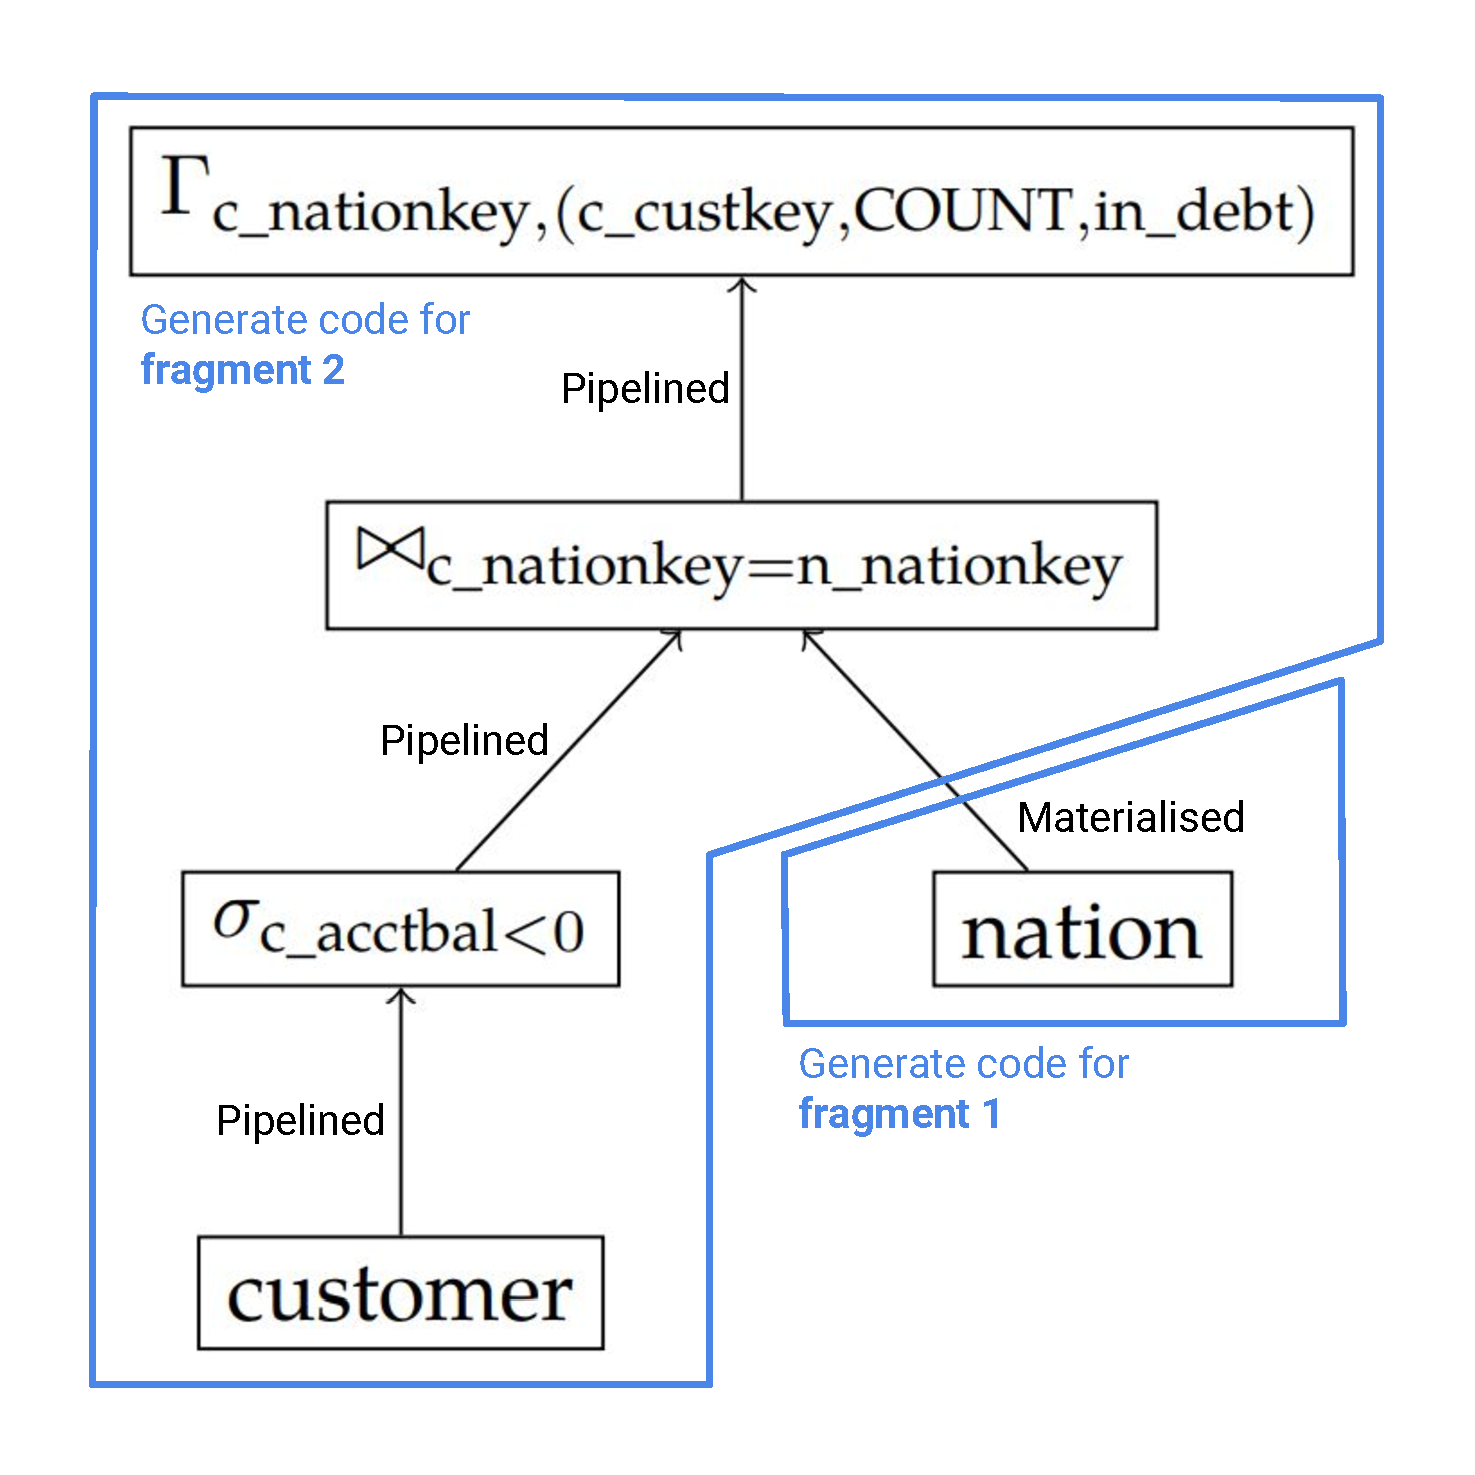
\includegraphics[width=0.9\linewidth]{introduction/codegen.pdf}
    \caption{Evaluating \ref{fig:simple-query} using code generation (the right input of the join would require its own fragment, if any operations were applied to the \texttt{nation} table)}
    \label{fig:code-generation}
\end{subfigure}
\caption{Approaches for improving query processing time}
\label{fig:improving-qpt}
\end{figure}

\emph{Voodoo} \cite{Pirk:2016:VVA:3007328.3007336} is a vector algebra which can be used as an intermediate representation between a database query and a code implementation, similar to what HyPer might produce. Voodoo allows the often data and hardware dependant kind of optimisations used in systems such as HyPer to be expressed in a portable way, and is designed to be \emph{tunable}, that is, it is able to express very simply most optimisations for in-memory query processing. It has been shown to generate highly-efficient OpenCL code to run on GPUs, outperforming existing state-of-the-art in-memory query processors for many queries.

\section{Motivation}

%Voodoo [https://pdfs.semanticscholar.org/45a9/1b4d9bcb2178c05e95685aca2f2aac94cdb0.pdf], is a high performance database kernel built around the idea of tunable, just-in-time compiled query execution. It is, arguably, the fastest database kernel right now. However, it is not a full data management system. It lacks an interactive query interface, a proper catalog manager, a logical query optimizer and many more components. In addition to that, it is built upon a fragile code generation process based on string concatenation. 

Whilst benchmarks have shown that using Voodoo allows some of the fastest query processing times out of any modern approach, it was not really available in a form that made it easy to use:

\begin{enumerate}
    \item The existing Voodoo implementation (detailed in \ref{original-voodoo-impl}) was a database \emph{kernel} meaning that it is far from being a full database management system.
    
    It was implemented as a replacement back-end for MonetDB. However the components to convert a query to a MonetDB plan remained separate to the Voodoo kernel itself, so there was no way to run queries, apart from TPC-H benchmarking queries, whose MonetDB plans were hard-coded into the driver program.
    
    \item The code generation itself was done by concatenating strings which formed the OpenCL program. This approach resulted in complex and fragile code, which was very difficult to extend. Importantly, once code had been written to the string, it could not be altered anymore so the program could only be written from top to bottom. This led to some optimisation strategies for the generated code being difficult or impossible to implement. 
    \item Certain parts of the code also suffered from particularly sparse documentation, and several bugs which were identified during this project.
\end{enumerate}

\section{Objectives}

This project essentially has two main goals: to replace the existing code generation engine with an AST based system (possibly using Clang) and provide an interactive SQL front-end using the Apache Calcite framework.

By achieving these objectives, we hope to extend the Voodoo project from a mere execution engine/kernel to something closer to a full database management system, thus lowering the barrier to entry.

We broke these goals down into three concrete tasks:
\begin{enumerate}
    \item \label{obj1} Build a front-end to firstly convert from an arbitrary SQL query (input by the end user) to a Calcite logical plan, and then from the logical plan to Voodoo vector algebra.
    \item \label{obj2} Create a new back-end that generates OpenCL code using an AST. The generated code should have an improved readability, and the back-end should be well tested and extensible.
    \item \label{obj3} Make Voodoo open for modification and further research by ensuring we have sufficient documentation on all aspects of the project.
\end{enumerate}

\section{Achievements}

\begin{enumerate}
    \item \textbf{Developed an Apache Calcite adapter for the Voodoo kernel}, which allows for any client to make queries using the Voodoo back-end via JDBC.
    
    \item \textbf{Built a new implementation of the Voodoo kernel} that uses a \textbf{Clang AST} to generate \textbf{cleaner OpenCL}.

    \item Built in support for \textbf{arbitrary database schemas} using the following types: \texttt{BOOLEAN}, \texttt{CHAR}, \texttt{INTEGER}, \texttt{BIGINT}, \texttt{DECIMAL}, \texttt{DATE} and \texttt{STRING}.
    
    \item \textbf{Support rule based logical plan optimisations} using Apache Calcite.
    
    \item \textbf{Lowered the barrier to entry} to the project for developers and users.
    
    \item Prepare \textbf{future extensions for generating C-like languages} such as CUDA and C++ using the Clang AST.
    
    \item \textbf{Created a graphical web interface} which could be used for testing or educating about the processing model of Voodoo, by showing intermediate representations when executing some SQL query.
\end{enumerate}

% 1. Document and formalise installation...

% 1a. Contribute bugfixes required to get code to compile and run, update documentation

% 1b. Provide a dockerfile that prescribes the required setup and that is used for the CI

% 1c. Introduce CI that ensures the project can always build

% 2. Develop Calcite adapter that supports SQL queries...

% 2a. Support arbitrary schemas with these types compared to before... (this was mentioned as extension in the original description of the project as \emph{catalog})

% 2b. Support arbitrary queries using these logical operators compared to before...

% 2c. Support rule-based logical optimisations using Calcite...(that was mentioned as extension in the original description of the project)

% 2d. Support enumerable operators using Calcite...

% 2e. Support integration with C++ printer implementation...

% 2f. Support integration with C++ AST implementation, by extending API...

% 2g. Provide a JDBC connection through Calcite

% (2h. Provide a front-end that demonstrates the full process).

% 3. Develop a Clang-AST based implementation of Voodoo API.

% 3a. Support these Voodoo operators compared to before...

% 3b. Improve quality of implementation code as measured by this metric...

% 3c. Improve quality of generated code as measured by this metric...

% 3d. Improve ease-of-use as demonstrated by example (cross?), by providing AST components...

% 3e. Support future extension to C-like languages such as CUDA / C++ through generic processing class... (GPU databases research too)

% 4. As an extension, the visualisation tool is perfect :wink:

% 4.a Debug tool..? Helps tune everything and much much research can come out of this like "what if the partition here used 0s instead of 1s?" wooow

% 4.b Educational purpose. Good vertical slice into a database with a quite unconventional processing model. Exposes the limitations of current popular systems and down to like what could be hand written code for the query; all that while making it visual, attractive and interative.

%%%%%%%%%%%%%%%%%%%%%%%%%%%%%%%%%%% MIKE's shit %%%%%%%%%%%%%%%%%%%%%%%%%%%%%%%%%%%%%%%%%%%%%%%%
% TODO: put this where it actually belongs (probably achievements sections), because we didn't start from scratch we probs don't want to strictly stick to the regular structure so that we can tell our story better


%%%%%%%%%%%%%%%%%%%%%%%%%%%%%%%%%%%% END OF MIKE's shit %%%%%%%%%%%%%%%%%%%%%%%%%%%%%%%%%%%%%%%%%%%%%%%%

\chapter{Design and Implementation}

Use \url{https://docs.google.com/document/d/1tCYCOFDeL8E3USIOunRNrqh6ekP_-kAQVHMrNJ4jk04} and the source code to complete. This section will probably need extensive, in-depth discussion of the algorithms we use, supported by diagrams for each part...

Should include discussion of technical challenges...

\section{Background}

\subsection{Architectural overview}

Diagram...

A full example query...

These are the components and their interactions...

Before vs after...

\subsection{Voodoo vector algebra}

This is what Voodoo is, how it works, and what it does (use \url{http://www.vldb.org/pvldb/vol9/p1707-pirk.pdf})...

Talk about existing architecture using monetdb and printer/planeater...

\subsection{Apache Calcite}

\emph{Apache Calcite} \cite{Begoli:2018:ACF:3183713.3190662} is a software framework that provides query language support, query optimisation and query processing, and is used by several popular data processing systems.

Whilst Calcite is written entirely in Java, which makes interaction with the Voodoo kernel difficult, Calcite was chosen as the framework on which to develop our front-end, thanks to its fairly widespread adoption, open-source friendliness and stability. By building on top of Calcite, we benefit from not having to entirely implement SQL parsing and validation, JDBC compliancy, and default operator implementations (which are useful when the Voodoo implementation of an operator would be beyond the scope of this project) ourselves.

\subsubsection{Architecture of Apache Calcite}

\begin{figure}
\includegraphics[width=0.5\textwidth]{design-and-implementation/calcite-architecture.png}
\centering
\caption{Architecture of Apache Calcite \cite{Begoli:2018:ACF:3183713.3190662}}
\label{fig:calcite-architecture}
\end{figure}

Calcite consists of most of the components needed to make a DBMS, with three significant omissions: algorithms to process data, storage of data, and a catalog for metadata. Figure \ref{fig:calcite-architecture} shows an overview of its architecture and interactions.

Firstly, Calcite provides a JDBC server (\emph{Avatica}), as well as a default implementation of its SPI. Alternatively, an application can use Avatica's JDBC driver directly (which is the approach we take with our web-interface).

Calcite then supports query evaluation in each of the following stages:
\begin{enumerate}
    \item \textbf{Parsing} the SQL query. Calcite provides an LL($k$) parser generated by JavaCC, and developers usually need not consider this step beyond setting some basic configuration options.
    \item \textbf{Validating} the SQL query. Calcite validates queries against any known metadata. Developers need to provide an interface that allows Calcite to get this metadata for a table (an \emph{adapter}).
    \item \textbf{Optimising} the logical plan, and converting it to physical expressions. Calcite can do this with some help. It provides two algorithms for rule-based logical query optimisation, as well as around one-hundred rules. However, developers will likely need to add further rules, including rules to rewrite a logical plan into physical expressions for their application.
    \item \textbf{Executing} the physical plan, by converting it into application-specific executions. Calcite can handle this in simple cases, say where the application actually supports SQL input (i.e. Calcite is just being used as an optimiser). In other cases, such as ours, this step requires a lot of application-specific code to be written.
\end{enumerate}

\subsubsection{Relational algebra}

Calcite uses relational algebra \cite{Codd:1970:RMD:362384.362685} to express queries. Specifically, it builds a tree of \texttt{RelNode}s, each of which represent a relational operator. Each \texttt{RelNode} could represent, for example, a \texttt{TableScan}, \texttt{Project}, \texttt{Filter}, \texttt{Aggregate}, \texttt{Join}, \texttt{Union}, \texttt{Intersect} or \texttt{Sort}.

Projection and sort fields, as well as filter and join conditions, are expressed by trees of \texttt{RexNode}s. A \texttt{RexNode} represents a row-level expression, and its implementations include \texttt{RexCall} (an operation such as "add" or "is equal to"), \texttt{RexInputRef} (a reference to an input column) and \texttt{RexLiteral} (a literal value), as well as many others (which we do not consider).

Relational expressions are associated with \emph{traits} (\texttt{RelTrait}s), which describe their physical properties, such as ordering, grouping, or partitioning. The most important trait, however, is the \emph{calling convention} (\texttt{Convention}), which specifies the data processing system where the expression will be executed. The \texttt{Logical} calling convention is used when no implementation has been selected.

\subsubsection{Query processing and optimisation}

Calcite includes \emph{planner rules} (\texttt{RelOptRule}s) to transform expression trees. Each rule defines a condition on the original tree, and a conversion, that rewrites part of the tree. Calcite provides common rules, such as the \texttt{FilterIntoJoinRule}, which pushes a filter into a join where possible, to reduce the work in the join. Developers also must provide their own rules to transform the tree from a logical to an optimised physical plan.

Calcite also provides two planner engines (\texttt{RelOptPlanner}s) to apply these rules: one requires a cost-model and uses a dynamic programming algorithm, similar to Volcano's \cite{Graefe:1994:VEP:627290.627558} (\texttt{VolcanoPlanner}), whilst the other exhaustively applies rules until it reaches a fixpoint (\texttt{HepPlanner}).

\subsubsection{Adapters}

As Calcite does not include a storage layer, it requires developers to build an \emph{adapter}. Figure \ref{fig:calcite-adapter} shows the design of a minimal adapter:
\begin{itemize}
    \item The \texttt{Model} is a JSON-formatted description of the physical properties of the data source being accessed.
    \item The \texttt{Schema} is a definition of the data found in the model, and is generated by a \texttt{SchemaFactory} for the adapter. Usually this will use a \texttt{TableFactory}, which generates a \texttt{Table} defining the names and types of the columns in each table, as well as any statistics available, such as cardinalities, distributions, and which columns are keys.
\end{itemize}

An adapter also usually provides a set of rules to be added to the planner. Specifically, rules to rewrite logical operators to physical operators of the adapter's convention.

The minimal rule set includes a translation for table-scans, which implement the access paths for tables in the adapter. Once Calcite can read the data, it can implement all other operators using the \texttt{Enumerable} calling convention, which uses a conventional iterator implementation written in Java.

Rules are also used to convert all other operators, to avoid plans relying too heavily on costly \texttt{Enumerable} operators. Each of these rules, in our case, defines an implementation instead using the \texttt{Voodoo} convention.

\begin{figure}
\includegraphics[width=0.5\textwidth]{design-and-implementation/calcite-adapter.png}
\centering
\caption{A minimal adapter for Apache Calcite \cite{Begoli:2018:ACF:3183713.3190662}}
\label{fig:calcite-adapter}
\end{figure}

\subsection{SWIG}

This is what SWIG is, how it works, and what it does (I guess \url{http://www.swig.org/Doc1.3/Java.html}?)...

\subsection{LibClang}

This is what LibClang is, how it works, and what it does (I guess \url{https://clang.llvm.org/doxygen/group__CINDEX.html}?)...

\subsection{OpenCL}

This is what OpenCL is, how it works, and what it does...

(CUDA?)

\section{Generating Voodoo from SQL using Apache Calcite}

Description of what Apache Calcite gives us...

\subsection{Defining schemas and importing data}

We don't have an explicit storage manager / catalog, so we use byte buffers...

We have a SchemaFactory which...

We have a TableFactory which then ... based on supported types...

\subsection{Translating logical operators to Voodoo}

Description of overall algorithm to convert logical plan -> voodoo (rules)...

For each logical operator, description of logical plan -> voodoo...

Using enumerables for other things...

\subsection{Translating row expressions to Voodoo}

Description of overall algorithm to convert row expression -> voodoo (visitor)...

For each row expression, description of expr -> voodoo...

\subsection{Communicating with the Voodoo Kernel}

Printer implementation...

Discussion of SWIG API...

How we pass values in for ClangAST implementation...

How we get values back for ClangAST implementation...

Technical challenges to do with garbage collection etc....

\subsection{Graphical web-interface}

We additionally provide a graphical front-end on top of our Calcite adapter, which displays the Calcite plan, Voodoo vector expressions, OpenCL and result for a query on the TPC-H schema.

\subsubsection{Purpose}

Building an interface was not an explicit goal of this project, and we do not expect it to be heavily used. However, the graphical web-interface's purpose is threefold:

\begin{enumerate}
\item It shows very clearly the transformations we make to generate OpenCL code from an SQL query, and provides graphical visualisations of the plan at various stages. As such, it is helpful for presenting the work we have done, and explaining how each intermediate representation is reached.
\item It provides a somewhat useful debugging interface. The alternative would be to use Apache Calcite's \texttt{sqlline} command-line interface. However, \texttt{sqlline} has several limitations. Firstly, there is a known issue whereby \texttt{sqlline} truncates long plans. Secondly, viewing the generated Voodoo vector expressions and the generated OpenCL require a different Voodoo implementations (\texttt{Printer} and \texttt{ClangAst} respectively), and hence different JDBC connections, which can be a little tedious to set up. The interface we have built does not require any such setup, and allows us to easily identify where a buggy query has gone wrong.
\item It proves that our database is JDBC-compliant, and provides sample Java code that includes connection configuration. It also shows how we can handle arbitrary SQL queries.
\end{enumerate}

\subsubsection{Implementation}

\begin{figure}
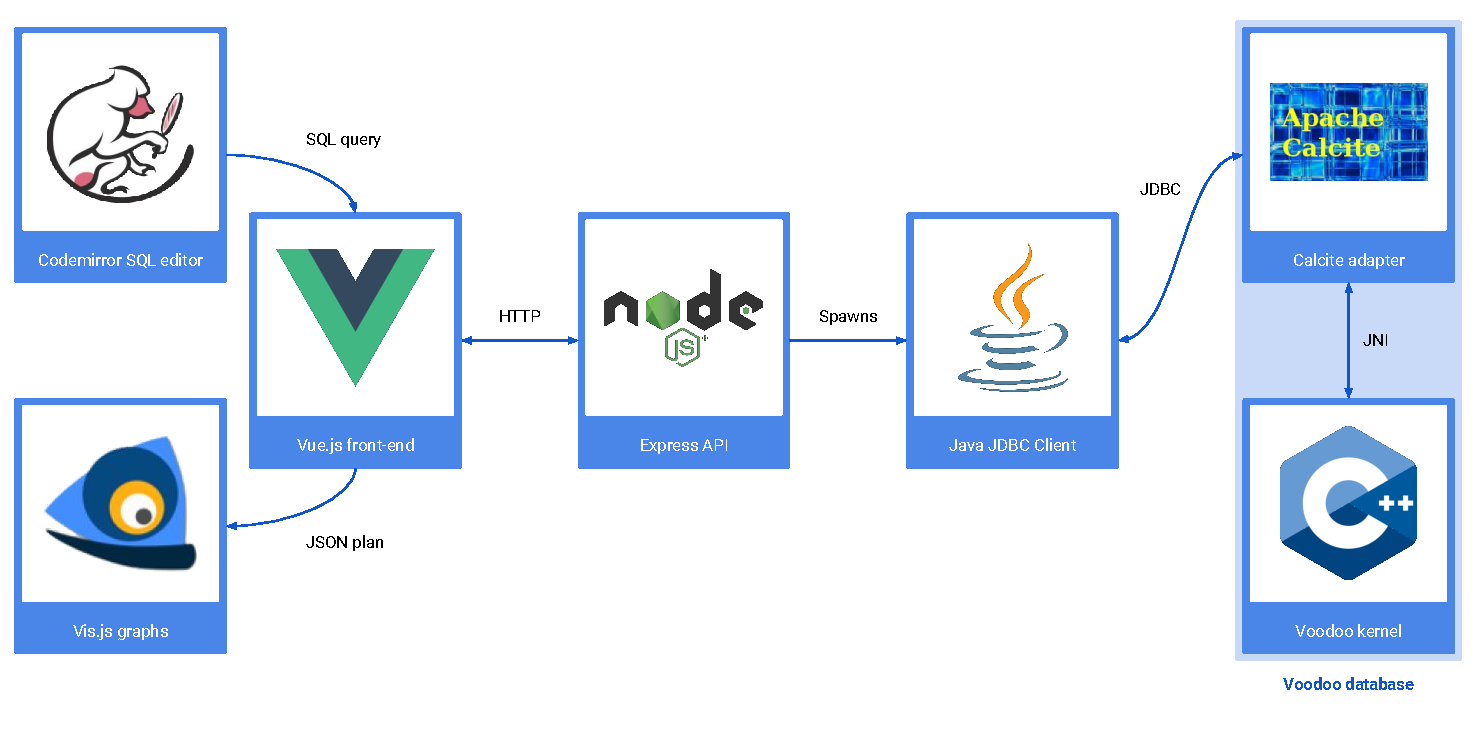
\includegraphics[width=\textwidth]{design-and-implementation/web-interface.pdf}
\centering
\caption{Architecture of the graphical web-interface}
\label{fig:web-interface}
\end{figure}

Figure \ref{fig:web-interface} shows the main components of the web-interface. Since this interface is not considered to be a real deliverable of this project, we favoured design decisions that allowed the most rapid development. As such we have:

\begin{enumerate}
\item A JDBC client, written in Java, that connects to our Voodoo implementation via the Calcite adapter. Note that the client never interacts directly with the Voodoo kernel, and so we rely on the kernel outputting Voodoo and OpenCL code, in addition to returning a result via the Calcite adapter. This approach provides a much cleaner interface than using an existing client, say \texttt{sqlline}, and avoids using unmaintained Node.js JDBC libraries.
\item An Express API, which accepts HTTP \texttt{GET} requests for a query. It returns a JSON, built from the output of the JDBC client, containing the plan, Voodoo, OpenCL and result for a query as well as any warnings or errors reported. This approach was much faster than using one of Java's more verbose HTTP server frameworks.
\item A Vue.JS frontend, which uses CodeMirror to provide an editor with SQL syntax highlighting and autocompletion. Queries are sent to the API, and we parse the response, using a hierarchical depth-first search starting from the returned vector, to build up the list of nodes and edges in a connected graph of the plan. The distances from the returned vector are used to define the $y$-coordinates ("levels") of operator nodes in the final graph, and vis.js then calculates $x$-coordinates using a physics simulation with spring forces between nodes.
\end{enumerate}

\section{Generating OpenCL from Voodoo using LibClang}

\subsection{Using LibClang to generate AST components}

We considered these options, and chose LibClang because...

For each component, description of how it is represented...

\subsection{Translating Voodoo to a Clang AST}

Description of overall algorithm to convert voodoo -> clang ast...

For each Voodoo API function, description of what it does and algorithm to convert it to AST...

\subsection{Generating and running OpenCL code}

Alternatives to OpenCL...

Generating fragments...

Running fragments...

Getting results...

\chapter{Project Management}

Use \url{https://docs.google.com/document/d/1tCYCOFDeL8E3USIOunRNrqh6ekP_-kAQVHMrNJ4jk04} to complete. Add screenshots/photos wherever possible...

\section{Project planning}

We originally decided on these checkpoint goals...
But actually achieved...

We split our work using GitLab issues, assigned to any group member...

We had these GitLab tags to keep track of issues in different milestones...

We attempted to split work equally, these were each person's main contributions...

\section{Project organisation}

We used eXtreme programming which means...

Meetings with Holger treated as iteration meetings, work estimation and backlog grooming...

Standups for more frequent communication...

Slack for all other communication, we used these channels...

\section{Software engineering practices}

Pair programming...

Use of Git, branching...

Testing...

CI...

PRs, requiring approval for pushes to Voodoo and Calcite repos...

\chapter{Evaluation}

\section{Deliverables}

\begin{enumerate}
    \item An \textbf{Apache Calcite adapter for the Voodoo kernel}, which allows for any client to connect to the Voodoo via JDBC.
    
    Previously, the TPC-H schema was hard-coded into the database, and only the pre-defined TPC-H SQL queries can be run. We now support arbitrary database schemas with the following types: \texttt{BOOLEAN}, \texttt{CHAR}, \texttt{INTEGER}, \texttt{BIGINT}, \texttt{DECIMAL}, \texttt{DATE} and \texttt{STRING}. Furthermore, we also allow execution of arbitrary SQL queries. For example, our unit tests for data-types uses non-TPC-H schema and queries.
    
    We currently support \texttt{TableScan}, \texttt{Project}, \texttt{Filter}, and in many cases we are also able to support \texttt{Aggregate} and \texttt{Join}. The only notable missing operation we do not support is \texttt{Sort}, but this can still be done through Calcite's \texttt{EnumerableSort} and not done in the Voodoo kernel. The same can be said about all other operators we do not support.
    
    \item A \textbf{new implementation of the Voodoo kernel} that uses a \textbf{Clang AST to generate OpenCL code}. This implementation is less fragile and complex than the existing string-based implementation. This can be shown in the metrics we generated on the previous implementation and our new implementation - table \ref{table:original-metrics} shows that the cyclomatic complexity of the previous implementation is \textbf{1.86} on average with a maximum of \textbf{71}, whereas ours is \textbf{1.05} with a maximum of \textbf{24}.
    
    In addition, our supervisor stated that our newly generated code was simpler and much nicer to work with when compared to the code generated in the old implementation, while performance remains roughly comparable to the previous implementation in most cases. We believe that it also significantly improves the extensibility of the Voodoo kernel.
    
    Finally, due to our generic class structure in the back-end, extending Voodoo to support the generation of C-like languages (such as CUDA and C++) can be achieved by small extensions to our back-end.
    
    \item A \textbf{usable product} with a low barrier to entry. We have formalised and automatically verify the installation process in a single \texttt{Dockerfile} that can serve as an install script for everything Calcite and Voodoo need. Furthermore we repeated and explained the installation steps in the README for better understanding and added support for Darwin systems. All this, along with the CI script file that document in detail the most up to date building and testing techniques and the CI log showing expected outputs, makes the project attractive to new comers and gives them more assurance to dive in deeper in it. 
    
    The project encourages extension too, with more than 80\% code coverage for both the Calcite adapter and our new back-end implementation (further details in appendix \ref{appendix:metrics}) and should therefore be appealing to researchers who want to explore Voodoo.
    
    \item A \textbf{logical query optimiser}. We use equivalence rules to optimise the Calcite logical plan that was generated from SQL.
    
    \item A \textbf{graphical web interface} as a way to demonstrate the architecture of the Voodoo project. The interface can show the intermediate representations when executing some arbitrary SQL query on the TPC-H schema (the Calcite logical plan generated from SQL, the Voodoo vector algebra generated from the logical plan, and the OpenCL generated using the new implementation of the back-end). Previously, no such interface existed.
\end{enumerate}

% We need to back all of these up with examples (demonstrate) or metrics (metric)...

% We can demonstrate how we have achieved our objectives and made it easier for researchers to use Voodoo...

% 1. Formalised, well-documented installation process (docker, CI, readmes etc.)

% - Before: didn't compile, easily broken, now: provably builds (demonstrate)...

% - Before: lacking documentation, now: largely documented (demonstrate)...

% 2. Calcite adapter allowing for arbitrary queries and schemas...

% - Before: hard-coded TPC-H schema, now: supports arbitrary schema with these types (demonstrate)...

% - Before: hard-coded int->query plan mapping, now: arbitrary SQL input with these commands, supporting JDBC (demonstrate)...

% - Support for these TPC-H queries (metric)

% - Support for these logical operators out of these possible ones (metric) + enumerable operators to plug the gap

% - Support for these row expressions out of these possible ones (metric)

% 3. Cleaner, better-documented, easier to use implementation of Voodoo API based on ASTs...

% - Improve quality of implementation code (demonstrate/metric)

% - Easier to build upon (demonstrate)

% - Improve quality of generated code (demonstrate/metric)

% - Support for these TPC-H queries (metric)

% - Support for these Voodoo API calls out of these possible ones (metric)

% - (If we have time) benchmark performance not significantly worse? (metric)

\section{Testing}

Overall description of testing framework, how we tested difficult parts... Description Of CI, Docker and how we run the tests

Since usability was at the centre of the 
Ease of user understanding, extension of the project was at the centre of this project and something that was integrated at each step of this. Testing had to not only be just part of our development cycle, it would be we would deliver 


\subsection{Continuous Integration}

Although continuous integration was a major point we had to deliver on, it was one of the trickiest one to maintain throughout the project and proved itself very time consuming, notably because of the time building each project takes. We are running the CI in parallel using multiple containers created from the original image. We originally used two different images for the calcite and voodoo repositories. This meant that extra deployment measures where at place, notably by publishing the SWIG library as a GitLab artifact\footnote{We needed to avoid publishing Voodoo publicly, that meant we couldn't use Maven's prefered solution which is the central repository.} from the master branch of the voodoo project to download from the calcite repository. 

The use of the single vertical Docker image from the Dockerfile made it possible to integrate voodoo as a submodule of calcite, and to move the integration tests within the adapter package. Furthermore it is then easy to cache the SWIG bindings generated for the submodule commit along with the Maven dependencies and the relevant calcite Maven modules which brought the building time (without tests) of the front-end down to 3 minutes for the adapter with calcite-core and LINQ4J.

The CI for calcite is very simple, the 3 targets for the SWIG bindings, the original \texttt{Driver} program, and the \texttt{runUnitTests} executable to run the \texttt{ClangAst} tests. We can note that it means our CI servers must have an OpenCl compatible device.

\subsection{Back-end}

Initially, test cases for each TPCH query were present, however the majority of tests executed with exceptions or failed to assert any conditions. We have implemented small feature tests for Voodoo operators like \texttt{CrossTest}, \texttt{foldSumTest}. These tests execute a minimal hand written query on a minimal dataset and check for correct behaviour of the specified operator. In addition, tests for TPCH Q6, Q19 and Q1 have been generated by the front end and translated into a test case, operating on a minimal data set and checking for correct output based on the original SQL query. Finally to help us come up with correct fragment resolution algorithms we used tests for important parts of the algortihms and edge cases (like \texttt{CanMergeDepedentFragments}, \texttt{CanMergeIndependentFragmentsFromMultipleTables}, etc.). 

The overall code coverage of 82\% with further details given in appendix \ref{appendix:metrics}. This result is notably brought down by having some voodoo operators not being implemented and therefore not tested, specific requirements for SWIG (like explicit default constructors and destructors, which do not represent features to test), and glue code called in the integration tests only which are not shown in either test coverage report. However, this is a great improvement compared to the original code, notably since those tests are feature oriented and tailored to fail on specific parts which should help beginners on the project to extend the code safely. This makes the codebase more friendly to contribution from other researchers, one of the major objectives of this project.

\subsection{Front-end}

We have those kind of test....


\subsection{Rename this section?}

We have already talked about the technical details and what they've achieved for both objectives \ref{obj1} and \ref{obj2}

A main objective (\ref{obj3}) for this project was to make Voodoo accessible, we brought in lots of new components that were potentially dangerous for that but we lowered the difficulty and thing:

Main problem being documentation (or lack of) for all the technology we use:

\begin{enumerate}
    \item Make familiar wrappers around clangAst because the doxygens are simply yuck
    \item Calcite's documentation is mostly just Javadocs and most things in the repo are quite obscure/experimental $\rightarrow$ we use only the most stable parts of calcite, make use of familiar Java patterns (\texttt{XXXFactory}, singleton for the API ;))) soon, ); make sure we can always pull from upstream to be latest bug fixes (calcite is in active development and constant expansion) by sticking to Apache's maven;s conventions, as hard as it is and not modifying existing code to avoid conflicts.
    \item This report will hold documentation for the back-end. it was written in a way that is extensible with reusable components with low coupling which was the major problem before
\end{enumerate}

\subsubsection{Diversity requirements for users (TODO dat)}

We provide extensive documentation to allow users to install and use Voodoo on any Unix-based systems. In addition, the documentation for 3rd party products required or used by Voodoo also support Unix-based systems.

We have taken some technology decisions to support equality. Currently the front-end can easily be replaced with one that an international users might use or are familiar with, since all that is required is an SQL client which can connect to our Calcite Voodoo adapter through JDBC, or using Avatica to build an ODBC driver.

Our documentation is currently in English, and there are 3rd party products which are only documented in English. However, it is the responsibility of the 3rd party owners to translate their documentation, and we can easily generate further translations using e.g. Google Translation.

Our product is mainly focused towards researchers, to allow them to experiment with generating Voodoo code. The subsection of users who can contribute and work on the project is restricted by our language choices. Those familiar with SQL and the languages used to build the product (Java, C/C++) should be able to work on and improve the project. As the front-end and back-end are separate repositories and systems, this does allow users to focus on only one side and therefore removes some of the language knowledge required to contribute to Voodoo.

\chapter{Reflection and Future Extensions}

\section{Significant technical challenges}

1. Gaining initial understanding of the code, and in particular, the Voodoo API commands, understanding original architecture, getting it to compile, sparse documentation/testing...

2. Using Calcite to generate API calls, involves traversing RexNodes etc, much more difficult than standard string-based approaches, not really done before (example)

3. Using SWIG, difficulties with API and maintaining backward-compatibility, type information, Java/C++ memory issues...

4. Using LibClang to build an AST (not really done before, as far as we are aware?)...

5. Handling strange codegen edge-cases in the back-end (give example)

Through these challenges we learned:

1. How to navigate complex existing codebases

2. How to manage technical debt and prioritise tasks in order to be able to demonstrate something impressive at the end of each iteration

\section{Legal and ethical issues}

Needs to be open-sourced -> implies understandable, easy to pick-up, use, contribute...

- Dependency / licensing issues...

Usefuleness:

- Very brief discussion of how high-performance databases are used, how they might be helpful to some and harmful to others...

\url{https://docs.google.com/document/d/10cTMsjru-TEgwY2nbnCN6L2P0eeM0OzeK3OvNSDzub0}:

- Designed for usability: easy to setup and use for researchers, documented etc. (need to know SQL and linux)

\url{https://docs.google.com/document/d/17c1YUBFDTNWwSnqsoz5ex1zbHZ30U1JQdMT_dVWceGQ}:

- Security: dependencies, code may be buggy / poorly documented in places...

- Reliability + support: dependencies, testing, documentation, issues

\section{Areas for future improvement and extension}

\subsection{Storage manager and catalog}

Voodoo doesn't have one... but it really should to be a proper DBMS...

It might look like this...

How this would affect the front end...

\subsection{Top-N queries}

Difficulty of sorting / top-N on graphics cards (\url{http://anilshanbhag.in/static/papers/gputopk_sigmod18.pdf})

\subsection{SWIG API design}

Look at the design for SWIG API now...

Difficulties this creates / measure coupling...

We would propose to...


\bibliographystyle{alpha}
\bibliography{bibs/references}

\appendix

\chapter{An Example: TPC-H Query 6}
\label{appendix:full-query}

TPC-H query 6 is arguably the simplest of the 22 queries in the TPC-H benchmark. In this section, we will show how our query processor evaluates this query, and the various intermediate representations that are reached.

Figure \ref{fig:q6-sql} shows the SQL query that is inputted. This corresponds to box 1 in figure \ref{fig:translation-process}.

\begin{figure}[H]
    \centering
    \begin{tabular}{|c|}
    \hline
    \begin{lstlisting}[language=SQL]
SELECT
    sum("l_extendedprice" * "l_discount") as "revenue"
FROM
    "lineitem"
WHERE
    "l_shipdate" >= date '1994-01-01'
    AND "l_shipdate" < date '1994-01-01' + interval '1' year
    AND "l_discount" between 0.06 - 0.01 AND 0.06 + 0.01
    AND "l_quantity" < 24
    \end{lstlisting} \\
    \hline
    \end{tabular}
    \caption{TPC-H query 6 in SQL}
    \label{fig:q6-sql}
\end{figure}

\newpage

The first step is to generate a plan for this query, corresponding to box 2 in figure \ref{fig:translation-process}. This query is initially parsed into a very simple logical plan, shown in figure \ref{fig:q6-logical-plan}. This plan first does a table scan of the \texttt{lineitem} table, then a selection (\texttt{WHERE ...}), then a projection (of \texttt{l\_extendedprice * l\_discount}), and finally an aggregation (performing the \texttt{sum}).

Due to the simplicity of the initial plan, there is not a lot of optimisation we can do. As such, the plan is almost identical after rule-based logical optimisation, as you can see in figure \ref{fig:q6-optimal-plan}. However, we have recognised that we are capable evaluating the full query, and so every operator has been assigned a \texttt{Voodoo} calling convention.

\begin{figure}[H]
    \begin{subfigure}{0.49\textwidth}
        \centering
        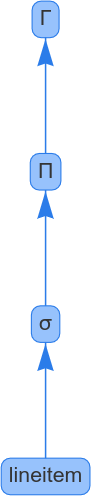
\includegraphics[width=0.15\linewidth]{appendix/q6-logical-plan.png}
        \caption{Initial logical plan (before rule applications)}
        \label{fig:q6-logical-plan}
    \end{subfigure}
    \begin{subfigure}{0.49\textwidth}
        \centering
        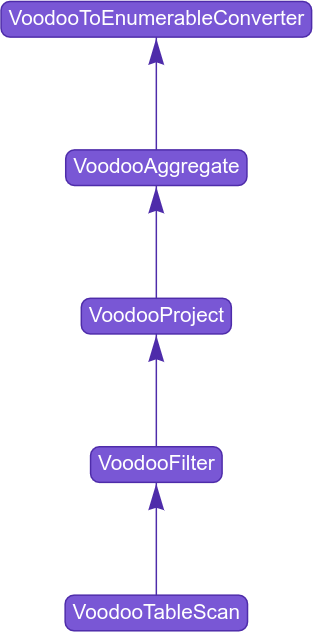
\includegraphics[width=0.45\linewidth]{appendix/q6-plan.png}
        \caption{Optimised plan (after rule applications)}
        \label{fig:q6-optimal-plan}
    \end{subfigure}
    \caption{Calcite plan for TPC-H query 6}
    \label{fig:q6-plan}
\end{figure}

One thing that cannot be seen in the graphical representation of the plans in figure \ref{fig:q6-plan} are the row expressions, of which there are two. One represents the filter condition, shown in figure \ref{fig:q6-rex}, and the other represents the single projection, \texttt{l\_extendedprice * l\_discount}. During the logical optimisation stage, we apply rules to reduce constants in these row expressions, as shown.

\begin{figure}[H]
    \definecolor{light-purple}{RGB}{186, 161, 201}
    \definecolor{light-blue}{RGB}{187, 211, 249}
    \definecolor{light-red}{RGB}{255, 165, 165}
    \begin{subfigure}{0.98\textwidth}
    \begin{tikzpicture}[
        ->,
        level distance=1.2cm,
        every node/.style={shape=rectangle, draw, align=center},
        level 1/.style={sibling distance=3.4cm},
        level 2/.style={sibling distance=1.7cm}, 
        level 3/.style={sibling distance=0.85cm},
    ]
        \node[fill=light-purple] {AND}
            child { node[fill=light-purple] {>=}
                child { node[fill=light-blue] {\texttt{l\_shipdate}} }
                child { node[fill=light-red] {8766} }}
            child { node[fill=light-purple] {<}
                child { node[fill=light-blue] {\texttt{l\_shipdate}} }
                child { node[fill=light-purple] {$+$}
                    child { node[fill=light-red] {8766} }
                    child { node[fill=light-red] {12} }}}
            child { node[fill=light-purple] {>=}
                child { node[fill=light-blue] {\texttt{l\_discount}} }
                child { node[fill=light-purple] {$-$}
                    child { node[fill=light-red] {6} }
                    child { node[fill=light-red] {1} }}}
            child { node[fill=light-purple] {<=}
                child { node[fill=light-blue] {\texttt{l\_discount}} }
                child { node[fill=light-purple] {$+$}
                    child { node[fill=light-red] {6} }
                    child { node[fill=light-red] {1} }}}
            child { node[fill=light-purple] {<}
                child { node[fill=light-blue] {\texttt{l\_quantity}} }
                child { node[fill=light-red] {24} }};
    \end{tikzpicture}
    \centering
    \caption{Before rule applications}
    \end{subfigure}
    \\ [5ex]
    \begin{subfigure}{0.98\textwidth}
    \begin{tikzpicture}[
        ->,
        level distance=1.2cm,
        every node/.style={shape=rectangle, draw, align=center},
        level 1/.style={sibling distance=3.4cm},
        level 2/.style={sibling distance=1.7cm}, 
        level 3/.style={sibling distance=0.85cm},
    ]
        \node[fill=light-purple] {AND}
            child { node[fill=light-purple] {>=}
                child { node[fill=light-blue] {\texttt{l\_shipdate}} }
                child { node[fill=light-red] {8766} }}
            child { node[fill=light-purple] {<}
                child { node[fill=light-blue] {\texttt{l\_shipdate}} }
                child { node[fill=light-red] {9131} }}
            child { node[fill=light-purple] {>=}
                child { node[fill=light-blue] {\texttt{l\_discount}} }
                child { node[fill=light-red] {5} }}
            child { node[fill=light-purple] {<=}
                child { node[fill=light-blue] {\texttt{l\_discount}} }
                child { node[fill=light-red] {7} }}
            child { node[fill=light-purple] {<}
                child { node[fill=light-blue] {\texttt{l\_quantity}} }
                child { node[fill=light-red] {24} }};
    \end{tikzpicture}
    \centering
    \caption{After rule applications}
    \end{subfigure}
    \centering
    \caption{Row expression for TPC-H query 6's filter condition}
    \label{fig:q6-rex}
\end{figure}

\newpage

The next stage of evaluation is to actually implement the plan in Voodoo algebra. This corresponds to box 3 in figure \ref{fig:translation-process}. By traversing the plan tree and the two row expression trees using visitor patterns, we produce the Voodoo algebra shown in figure. \ref{fig:q6-voodoo}.

\begin{figure}[H]
    \centering
    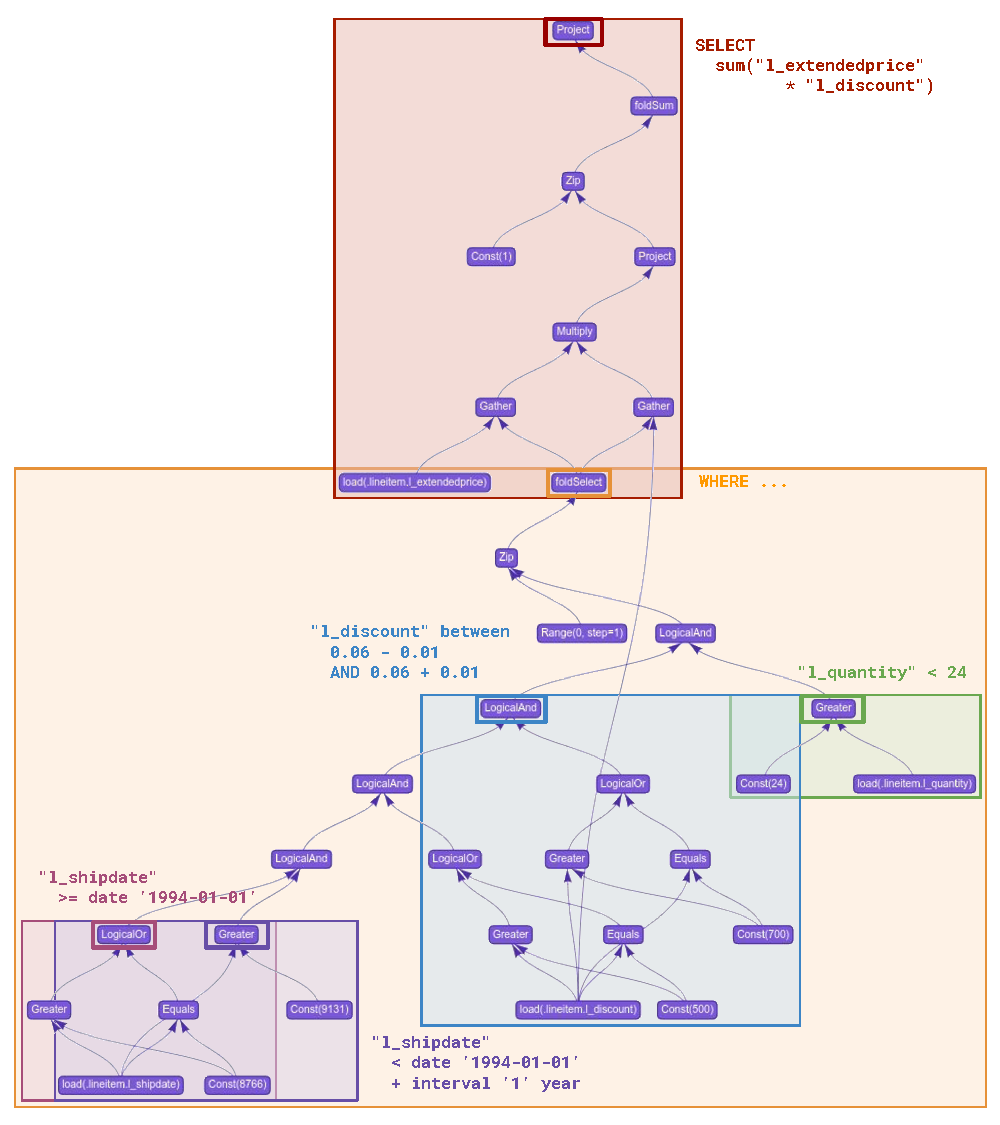
\includegraphics[width=\linewidth]{appendix/q6-voodoo.pdf}
    \caption{Voodoo vector expressions generated for TPC-H query 6}
    \label{fig:q6-voodoo}
\end{figure}

\newpage

Finally, we use these Voodoo API calls to build a Clang AST, as shown in figure \ref{fig:q6-ast}. This corresponds to box 4 in figure \ref{fig:translation-process}.

\begin{figure}[H]
    \centering
    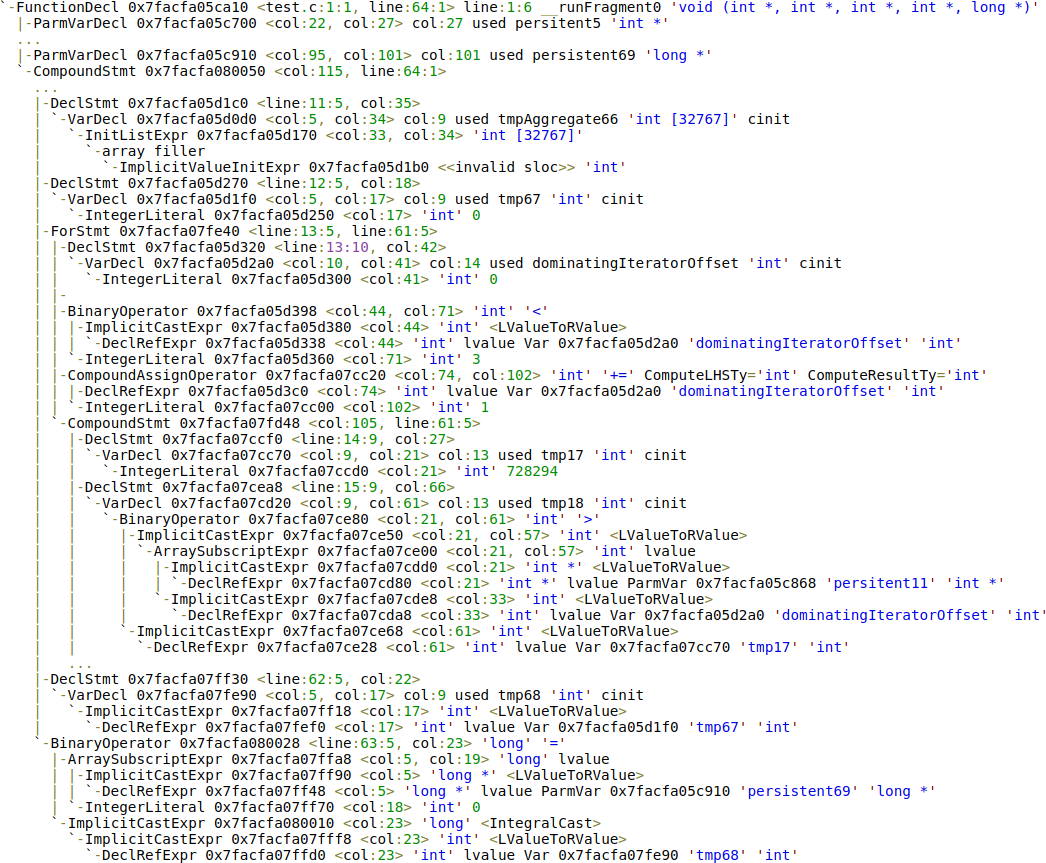
\includegraphics[width=\linewidth]{appendix/q6-ast.png}
    \caption{Part of the AST generated for TPC-H query 6}
    \label{fig:q6-ast}
\end{figure}

From the AST, we generate the OpenCL code, shown in figure \ref{fig:q6-opencl}. This corresponds to box 5 in figure \ref{fig:translation-process}. The only change we have made to this code is to move arguments onto the following lines where necessary.

\begin{figure}[p]
    \centering
    \begin{tabular}{|c|}
    \hline
    \begin{lstlisting}[language=C]
__kernel void __runFragment0(__global int *persitent6, __global int *persitent10,
                             __global int *persitent13, __global int *persitent15,
                             __global long *persistent63) {
    struct {
        int fold;
        int value;
    } tmp38;
    int tmp39;
    struct {
        int fold;
        int value;
    } tmp59;
    int tmpAggregate60[32767] = {};
    int tmp61 = 0;
    for (int dominatingIteratorOffset = 0;
             dominatingIteratorOffset < 309;
             dominatingIteratorOffset += 1) {
        int tmp17 = 8766;
        int tmp18 = persitent6[dominatingIteratorOffset] > tmp17;
        int tmp19 = persitent6[dominatingIteratorOffset] == tmp17;
        int tmp20 = tmp18 || tmp19;
        int tmp21 = 9131;
        int tmp22 = tmp21 > persitent6[dominatingIteratorOffset];
        int tmp23 = 500;
        int tmp24 = persitent15[dominatingIteratorOffset] > tmp23;
        int tmp25 = persitent15[dominatingIteratorOffset] == tmp23;
        int tmp26 = tmp24 || tmp25;
        int tmp27 = 700;
        int tmp28 = tmp27 > persitent15[dominatingIteratorOffset];
        int tmp29 = persitent15[dominatingIteratorOffset] == tmp27;
        int tmp30 = tmp28 || tmp29;
        int tmp31 = 24;
        int tmp32 = tmp31 > persitent10[dominatingIteratorOffset];
        int tmp33 = tmp20 && tmp22;
        int tmp34 = tmp33 && tmp26;
        int tmp35 = tmp34 && tmp30;
        int tmp36 = tmp35 && tmp32;
        int tmp37 = dominatingIteratorOffset + 0;
        {
            tmp38.fold = tmp37;
            tmp38.value = tmp36;
        }
        {
            tmp39 = tmp38.value ? tmp38.fold : -1;
            if (tmp38.value) {
                int tmp52 = persitent13[tmp39];
                int tmp54 = persitent15[tmp39];
                int tmp56 = tmp52 * tmp54;
                int tmp57 = tmp56;
                int tmp58 = 1;
                {
                    tmp59.fold = tmp58;
                    tmp59.value = tmp57;
                }
                tmp61 = tmpAggregate60[tmp59.fold]
                      = tmpAggregate60[tmp59.fold] + tmp59.value;
            }
        }
    }
    int tmp62 = tmp61;
    persistent63[0] = tmp62;
}
    \end{lstlisting} \\
    \hline
    \end{tabular}
    \caption{OpenCL code generated for TPC-H query 6}
    \label{fig:q6-opencl}
\end{figure}

\chapter{The Apache Calcite Framework}
\label{appendix:calcite}

\subsubsection{Architecture of Apache Calcite}

\begin{figure}[H]
\includegraphics[width=0.4\textwidth]{appendix/calcite-architecture.png}
\centering
\caption{Architecture of Apache Calcite \cite{Begoli:2018:ACF:3183713.3190662}}
\label{fig:calcite-architecture}
\end{figure}

Calcite consists of most of the components needed to make a DBMS, with three significant omissions: algorithms to process data, storage of data, and a catalog for metadata. Figure \ref{fig:calcite-architecture} shows an overview of its architecture and interactions.

Firstly, Calcite provides a JDBC server (\emph{Avatica}), as well as a default implementation of its SPI. Alternatively, an application can use Avatica's JDBC driver directly (which is the approach we take with our web-interface).

Calcite then supports query evaluation in each of the following stages:
\begin{enumerate}
    \item \textbf{Parsing} the SQL query. Calcite provides an LL($k$) parser generated by JavaCC, and developers usually need not consider this step beyond setting some basic configuration options.
    \item \textbf{Validating} the SQL query. Calcite validates queries against any known metadata. Developers need to provide an interface that allows Calcite to get this metadata for a table (an \emph{adapter}).
    \item \textbf{Optimising} the logical plan, and converting it to physical expressions. Calcite can do this with some help. It provides two algorithms for rule-based logical query optimisation, as well as around one-hundred rules. However, developers will likely need to add further rules, including rules to rewrite a logical plan into physical expressions for their application.
    \item \textbf{Executing} the physical plan, by converting it into application-specific executions. Calcite can handle this in simple cases, say where the application actually supports SQL input (i.e. Calcite is just being used as an optimiser). In other cases, such as ours, this step requires a lot of application-specific code to be written.
\end{enumerate}

\subsubsection{Relational algebra}
\label{rel}

Calcite uses relational algebra \cite{Codd:1970:RMD:362384.362685} to express queries. Specifically, it builds a tree of \texttt{RelNode}s, each of which represent a relational operator. Each \texttt{RelNode} could represent, for example, a \texttt{TableScan}, \texttt{Project}, \texttt{Filter}, \texttt{Aggregate}, \texttt{Join}, \texttt{Union}, \texttt{Intersect} or \texttt{Sort}.

Projection and sort fields, as well as filter and join conditions, are expressed by trees of \texttt{RexNode}s. A \texttt{RexNode} represents a row-level expression, and its implementations include \texttt{RexCall} (an operation such as "add" or "is equal to"), \texttt{RexInputRef} (a reference to an input column) and \texttt{RexLiteral} (a literal value), as well as many others (which we do not consider).

Relational expressions are associated with \emph{traits} (\texttt{RelTrait}s), which describe their physical properties, such as ordering, grouping, or partitioning. The most important trait, however, is the \emph{calling convention} (\texttt{Convention}), which specifies the data processing system where the expression will be executed. The \texttt{Logical} calling convention is used when no implementation has been selected.

\subsubsection{Query processing and optimisation}

Calcite includes \emph{planner rules} (\texttt{RelOptRule}s) to transform expression trees. Each rule defines a condition on the original tree, and a conversion, that rewrites part of the tree. Calcite provides common rules, such as the \texttt{FilterIntoJoinRule}, which pushes a filter into a join where possible, to reduce the work in the join. Developers also must provide their own rules to transform the tree from a logical to an optimised physical plan.

Calcite also provides two planner engines (\texttt{RelOptPlanner}s) to apply these rules: one requires a cost-model and uses a dynamic programming algorithm, similar to Volcano's \cite{Graefe:1994:VEP:627290.627558} (\texttt{VolcanoPlanner}), whilst the other exhaustively applies rules until it reaches a fixpoint (\texttt{HepPlanner}).

\subsubsection{Adapters}

\begin{figure}[H]
\includegraphics[width=0.42\textwidth]{appendix/calcite-adapter.png}
\centering
\caption{A minimal adapter for Apache Calcite \cite{Begoli:2018:ACF:3183713.3190662}}
\label{fig:calcite-adapter}
\end{figure}

As Calcite does not include a storage layer, it requires developers to build an \emph{adapter}. Figure \ref{fig:calcite-adapter} shows the design of a minimal adapter:
\begin{itemize}
    \item The \texttt{Model} is a JSON-formatted description of the physical properties of the data source being accessed.
    \item The \texttt{Schema} is a definition of the data found in the model, and is generated by a \texttt{SchemaFactory} for the adapter. Usually this will use a \texttt{TableFactory}, which generates a \texttt{Table} defining the names and types of the columns in each table, as well as any statistics available, such as cardinalities, distributions, and which columns are keys.
\end{itemize}

An adapter also usually provides a set of rules to be added to the planner. Specifically, rules to rewrite logical operators to physical operators of the adapter's convention.

The minimal rule set includes a translation for table-scans, which implement the access paths for tables in the adapter. Once Calcite can read the data, it can implement all other operators using the \texttt{Enumerable} calling convention, which uses a conventional iterator implementation written in Java.

Rules are also used to convert all other operators, to avoid plans relying too heavily on costly \texttt{Enumerable} operators. Each of these rules, in our case, defines an implementation instead using the \texttt{Voodoo} convention.

\chapter{Relational Operator Implementations}
\label{appendix:rel}

\begin{enumerate}
    \item \textbf{Table scans}
    
    \texttt{TableScan} is a relatively simple operator that can access a \texttt{VoodooTable}, and \texttt{Import}, \texttt{Persist} and \texttt{Load} its column vectors into the back-end's memory.

    \item \textbf{Projections}
    
    \texttt{Project} is a similarly simple operator. Each projected field is defined as a row expression and is implemented as described in subsection \ref{sub:rex}. The final result is then made available for the parent node to access.

    \item \textbf{Filters}

    \begin{figure}[H]
        \centering
        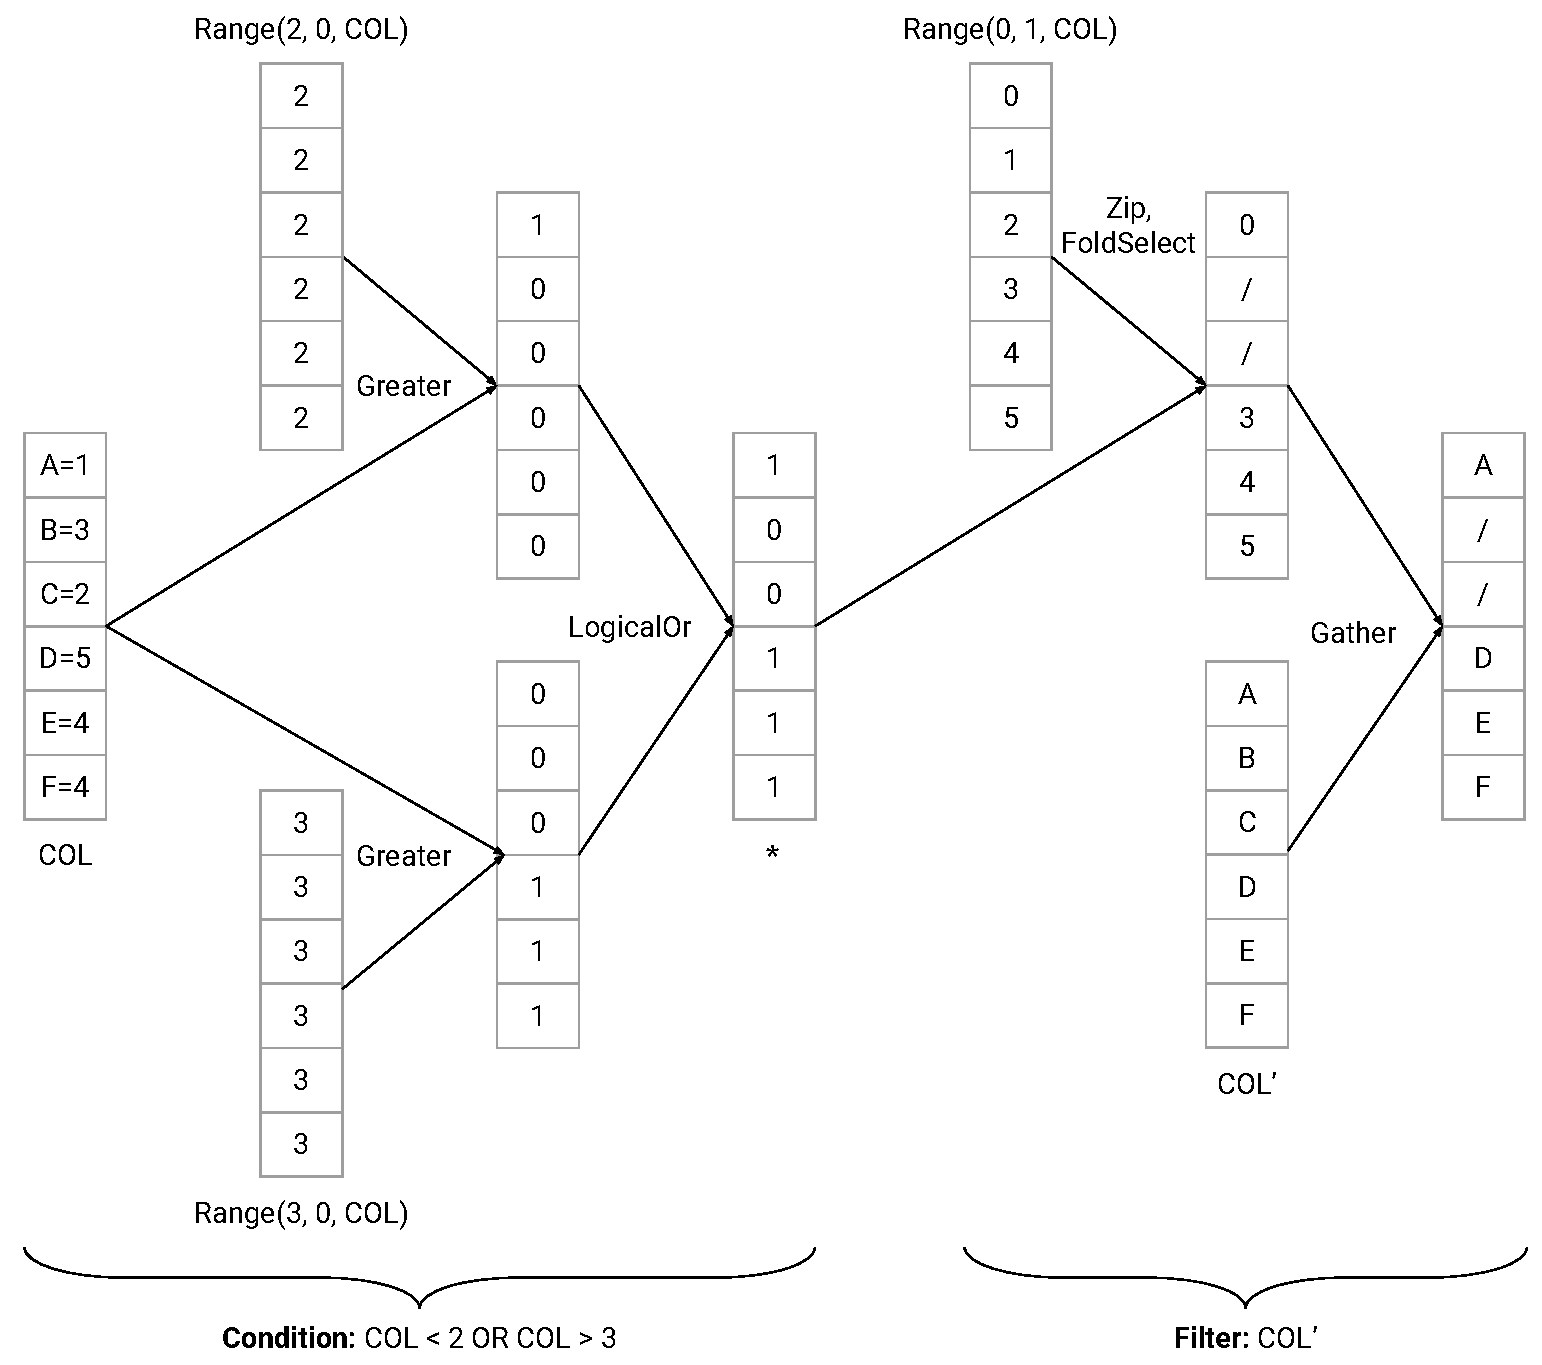
\includegraphics[width=0.75\linewidth]{appendix/filter.pdf}
        \caption{Implementing $\sigma_{\text{COL} < 2 \lor \text{COL} > 3}\text{COL}'$ in Voodoo vector algebra}
        \label{fig:filter}
    \end{figure}
    
    \texttt{Filter} represents a selection in relational algebra. To implement a filter, we first implement its condition, which is a row expression. This should return a vector of zeroes and ones, where the ones correspond to rows which should be selected. Figure \ref{fig:filter} shows an example of this, where we have reached the vector labelled "$*$". We \texttt{Zip} this condition vector with the row indices of the table. We then use a \texttt{FoldSelect}, which selects the indices corresponding to non-zero values in the condition vector. These indices are then used to \texttt{Gather} the selected rows from each column of the table.
    
    The final result has non-selected rows as empty-slots, shown as "$/$" in the figure. In reality, these are "junk" values, and are difficult to distinguish in some cases. As such, in addition to the resulting vectors, we always keep a reference to the condition vector ($*$), which allows us to determine exactly which rows were selected.
    
    \item \textbf{Aggregates}
    
    \texttt{Aggregate} represents a grouped aggregation in relational algebra. Currently, we support the \texttt{SUM}, \texttt{COUNT}, \texttt{MIN}, \texttt{MAX} and \texttt{AVG} aggregate functions applied without grouping (i.e. for the entire column). We will describe a \texttt{SUM} here, but it is clear to see that the other operators would be implemented similarly. To implement this operator, we must first implement the specified row expression, which should return a vector containing the values from the specified column with the expression applied to each value. We then \texttt{zip} this vector with a run-vector which contains all ones. A \texttt{foldSum} is then applied to this, which generates a new vector containing the sum of all the values in each run in the run vector (in this case, we have a single run, so all values are summed). Finally, we \texttt{project} this final vector onto the specified alias specified. Figure \ref{fig:aggregate} shows an example of this.
    
    \begin{figure}[H]
        \centering
        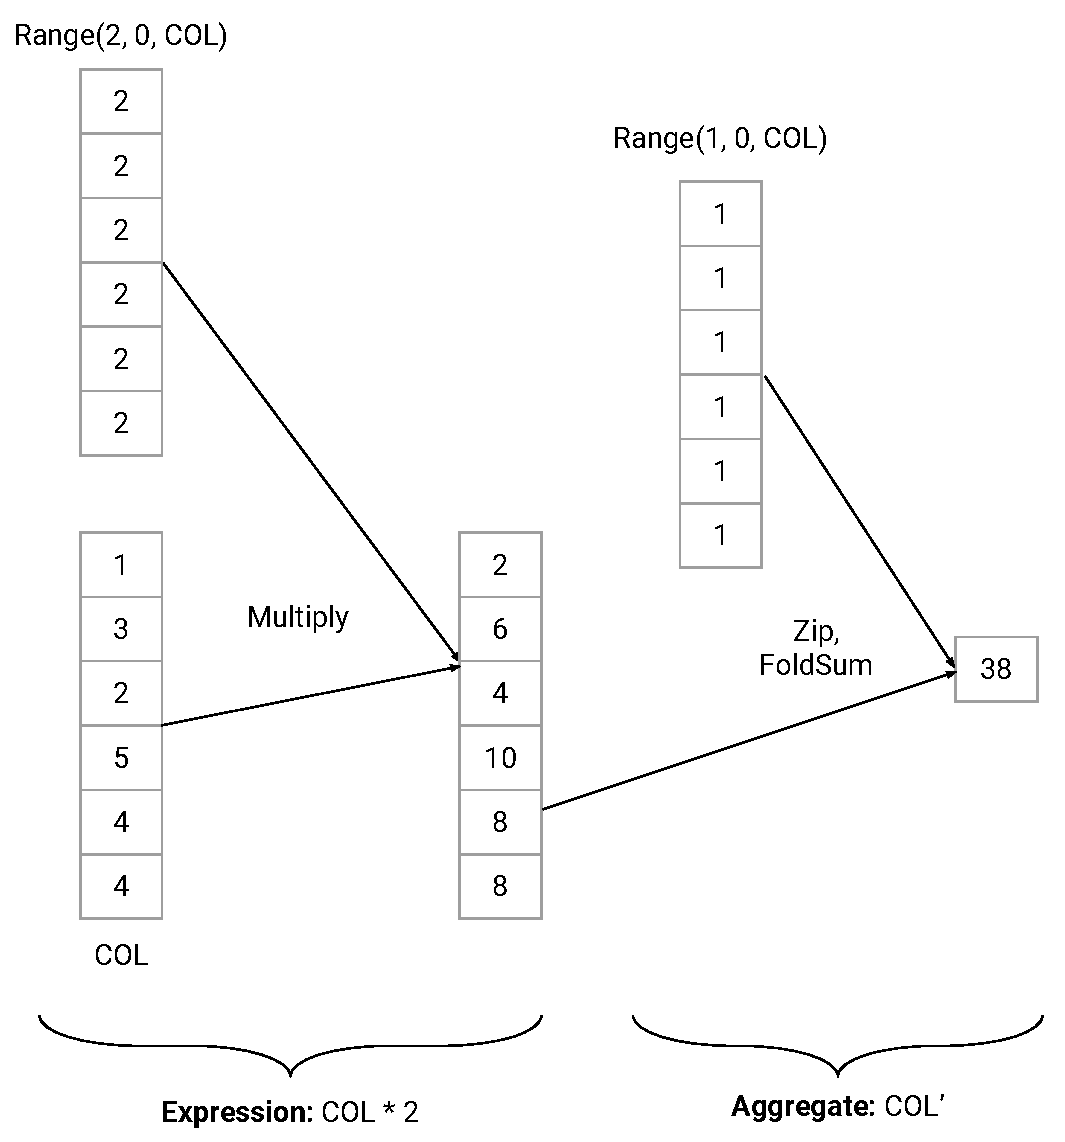
\includegraphics[width=0.5\linewidth]{appendix/aggregate.pdf}
        \caption{Implementing $\Gamma_{(\text{COL} \times 2, (\{\}, \texttt{SUM}))}$ in Voodoo vector algebra}
        \label{fig:aggregate}
    \end{figure}
    
    Although currently not fully implemented, supporting grouping would involve a \texttt{partition} of the group key\footnote{For multiple group keys, we need use \texttt{BitShift} and \texttt{BitwiseOr} operations to combine the group key vectors together as a single vector, and use this result as the group key.} using a vector of indices. We will call the result of this operation \texttt{A}. Then, we \texttt{scatter} the vector \texttt{A} with respect to the group key - let this result be the vector \texttt{B}. We also \texttt{scatter} the vector \texttt{A} with respect to the vector of values which we want to apply the aggregate function to - let this result be the vector \texttt{C}. After, we \texttt{zip} the vectors \texttt{B} and \texttt{C} and apply \texttt{foldSum} to this (now using \texttt{B} as the run-vector, instead of just a constant vector of ones). An example of this is shown in figure \ref{fig:group-by}.
    
    Since the empty slots in this case may be difficult to determine, we could \texttt{scatter} a vector of ones into a vector zeroes using the group key as the pivots, in order to produce a column allowing us to determine exactly which rows form the result.
    
    \begin{figure}[H]
        \centering
        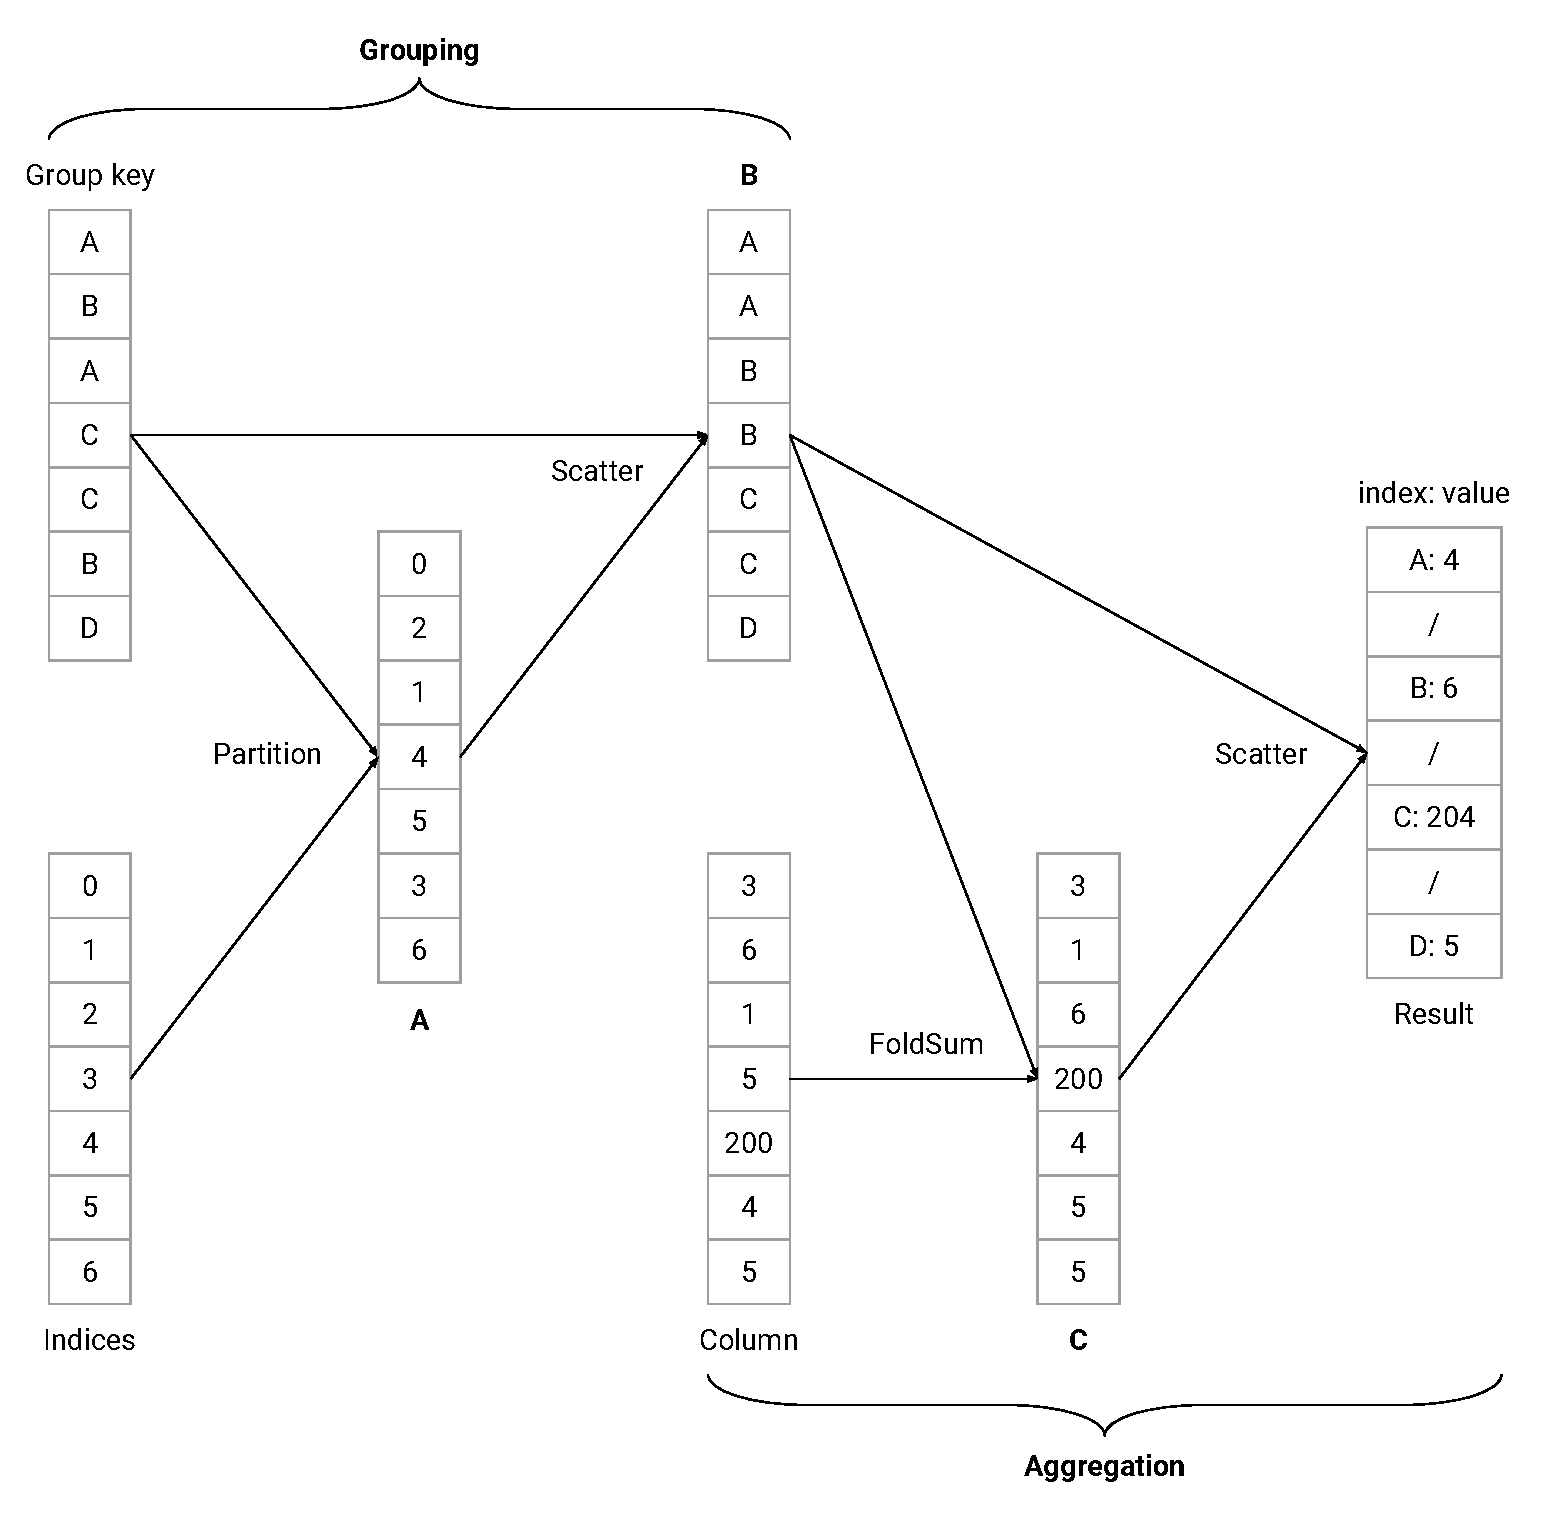
\includegraphics[width=0.75\linewidth]{appendix/group-by.pdf}
        \caption{Implementing $\Gamma_{(\text{Column}, (\text{Group key}, \texttt{SUM}))}$ in Voodoo vector algebra}
        \label{fig:group-by}
    \end{figure}
    
    \item \textbf{Joins}
    
    \texttt{Join} is a rather difficult operator to implement. We have currently implemented the most simple case, which is just a cross product (i.e. a join with no condition). We apply \texttt{Cross} to a vector from the first relation with a vector from the second relation. After, we use the result in a \texttt{Gather}, with the columns being projected. If the join has a condition, we can then apply the filter (see above) with the join condition.
    
    We also have an implementation which may be used when there is a foreign key relationship, referring to a primary key that is known to be dense. In this case, all that is required is to \texttt{Subtract} the offset of the dense key column, and apply a \texttt{Gather}.
    
    One thing to note is that if a join is performed on columns that have been filtered, it can be difficult to tell which rows should be returned in the final result. One solution is to never push filters inside joins, which would completely avoid this issue. Another is to use the condition columns, which \texttt{Filter}s keep a reference to, and apply \texttt{Gather}s and logical vector operations to work out which columns in the join result should be filtered.
    
\end{enumerate}

\chapter{Voodoo API Implementation}
\label{appendix:api}

\begin{enumerate}

\item \texttt{Import(vector v1)}

This loads a vector holding input data (in the form of a pointer to a buffer) into the \texttt{VectorProcessor}. This vector is now referred to as a persistent or input vector.

\item \texttt{Load(vector v1)}

This loads a previously created persistent vector and allows other calls to access the data held within it. It registers the persistent vector as being present in the parameters to the final fragment. 

This generates a \texttt{Clang::ParmVarDecl} declaring the name and type of the vector in the fragments function parameters.

\item \texttt{Project(vector v1, KeyPath k1)}

This projects a loaded vector and allows other calls to access the data held within it. It leads to the generation of the dominating iterator for loop that is used to cycle through the values of the projected vector. If the vector v1 contains multiple members, then KeyPath k1 is used to access the specific member, otherwise it is ignored.

This generates a \texttt{Clang::DeclStmt} declaring and initialising the vector. E.g.

{\centering\texttt{tmp1 = v1[dominatingIterator].k1}\par}

\item \texttt{Gather(vector v1, positions)}

\texttt{Gather} is a more complicated version of project. Instead of cycling through all the values of a vector it takes in another vector (positions) which it uses as the indices of the vector to access. 

This generates a \texttt{Clang::DeclStmt} declaring and initialising the vector. E.g. 

{\centering\texttt{tmp1 = v1[positions[dominatingIterator]]}\par}

\item \texttt{LogicalAnd(vector v1, v2)}, \texttt{LogicalOr(vector v1, v2)}, \texttt{BitwiseAnd(vector v1, v2)}, \texttt{BitiwseOr(vector v1, v2)}, \texttt{Equals(vector v1, v2)}, \texttt{Add(vector v1, v2)}, \texttt{Subtract(vector v1, v2)}, \texttt{Greater(vector v1, v2)}, \texttt{Modulo(vector v1, v2)}, \texttt{Divide(vector v1, v2)}

All of these Voodoo API calls take two vectors of identical size and perform a single operation on them, outputing a single vector of the same size. 

This generates a \texttt{Clang::DeclStmt} declaring and initialising the vector. E.g.

{\centering\texttt{tmp1 = v1 (+ / - / * / == / ...) v2}\par}

\item \texttt{BitShift(vector v1, v2)}

This take two vectors of identical size and shifts the first by the second amount. If the amount is positive it is a right shift otherwise it is a left shift. This outputs a single vector of the same size.

\item \texttt{Range(int/long/float min, count, step)}

\texttt{Range} generates a vector of size count, representing a range of numbers, starting at min and increasing by count between each number. Count can also be input as a vector, and range will generate a vector of identical size to count. 

This generates a \texttt{Clang::DeclStmt} declaring and initialising the vector. E.g.

{\centering\texttt{tmp1 = min + step * dominatingIterator}\par}

\item \texttt{Zip(vector v1, v2, KeyPath k1, k2)}

\texttt{Zip} takes two vectors of identical size and zips them together into one vector. The output vector will contain vector \texttt{v1} in KeyPath \texttt{k1} and vector \texttt{v2} in KeyPath \texttt{k2}. This is necessary for the fold operations, which require a zipped vector, and utilise KeyPath to access them.

This generates a \texttt{Clang::DeclStmt} declaring and initialising the vector. E.g.

{\centering\texttt{tmp1 = \{{k1: v1, k2: v2\}}}\par}

\item \texttt{FoldSelect(vector v1, KeyPath fold, val)}

\texttt{foldSelect} takes a vector and branches via an if statement based on the val of the vector. Returning \texttt{v1.fold} if \texttt{v1.val} is non-zero, otherwise returning -1. Any further statements using the output of the \texttt{foldSelect} will be placed inside the if statement.

This generates multiple \texttt{Clang::Stmts}, generating the output of the \texttt{foldSelect} and the branch:

{\centering\texttt{tmp4 = tmp3.value ? tmp3.fold : -1; if (tmp3.value) \{{...\}}}\par}

\item \texttt{FoldSum(vector v1, KeyPath fold, val)}, \texttt{FoldMax(vector v1, KeyPath fold, val)}, \texttt{FoldMin(vector v1, KeyPath fold, val)}

\texttt{foldSum}/\texttt{Max}/\texttt{Min} takes a vector and computes the sum / max / min of the val based on the fold attribute. This generates a \texttt{Clang::Stmt} assigning:

{\centering\texttt{tmp7 = tmpAggregate6[tmp5.fold] = tmpAggregate6[tmp5.fold] + tmp5.value;}\par}

This will "reduce" a vector to a single value. 

\item \texttt{Cross(vector v1, v2)}

\texttt{Cross} generates a nested for loop, looping through the values of \text{v2}. This allows data from one table to be crossed with another table. During the block generation process this manifests as a block contained within another block.

This generates a \texttt{Clang::Stmt} declaring the for loop:

{\centering\texttt{for(int dominatingIteratorOffset2 = 0; i < v2.size; i++) \{{...\}}}\par}

and allows future calls to access the new iterator to loop through the values of v2.

\item \texttt{ReturnVector(vector v1)}

\texttt{ReturnVector} projects a vector into a new output vector with a buffer to hold the final output values. This adds the output vector to the parameter list so the buffer location can specified at runtime by the \texttt{VectorProcessor}. This invokes the fragment generation code and generates the final code to be run in addition to the output size and type, storing it in the vector. This generates a \texttt{Clang::Stmt} assigning the vector. E.g.

{\centering\texttt{persistent1[0] = v1} or \texttt{persistent1[dominatingIterator] = v1}\par}

and a \texttt{Clang::ParmVarDecl} declaring the name and type of the vector in the fragments function parameters. This returns the vector, ready to be resolved (ran) and for the values to be read.

\item \texttt{ReturnMultiVector(list of vectors vs)}

This generates multiple return statements, adding each return statement to the fragment as well as each output buffer and then generating the code for this fragment. The final code is stored in the first vector. When the list of vectors is resolved, only the first vector is run, but all output buffers from the list are registered to OpenCL and so all output vectors are populated. 

This returns a list of vectors, ready to be resolved and for the values of each vector to be read.

\item \texttt{Resolve(vector or list of vectors)}

This runs the given vectors, passing input and output buffers to the \texttt{VectorProcessor} and then returning the vectors containing the results back to the user.

This call will only work on vectors produced from previous calls to \texttt{ReturnVector} or \texttt{ReturnMultiVector}.
 
Once the relevant Clang statements have been created, they are added to the \texttt{AstVector}. The \texttt{AstVector} also stores the \texttt{AstVector}s that this function requires.

\item \texttt{Partition(vector v1, vector v2)}

Partition takes an input vector v1 and a list of pivots v2. It loops through the input vector, and for each value, increment the size of the histogram bin the input belongs in. The semantics is defined such that the input value goes in the bucket that has a pivot greater the input value. Then iterate through the histogram array and work out the starting positions using a prefix sum and set the sizes back to zero. Each of these steps can be done in parallel. \cite{Maleki:2016:HTM:2980983.2908089}
Using the histogram start and size values, it returns the pivot that is assigned to the input vector. This essentially outputs the positions of the input values if they were ordered(\texttt{vector v3}). There are cases where this can be simplified.

An example of just the working out the pivot for the input value is presented below. 

{\centering\texttt{v3.val = v3Histogram[v1.val \& 31].start + v3Histogram[v1.val \& 31].size++;}\par}


\item \texttt{Scatter(vector v1, vector v2, vector v3)}
Scatter takes an input vector v1, an output vector v2 and a list of pivots v3. It loops through the values in input, placing them in the corresponding pivot position in the output vector. On conflict, values are overwritten in the output vector. Scatter breaks the current block, as a full iteration through the input vector is required to correctly generate the output vector. This generates a \texttt{Clang::Stmt} assigning the vector. E.g.

{\centering\texttt{v1[v2] = v3}\par}

\end{enumerate}

\chapter{Generating Blocks for \texttt{FoldSelect}}

Dealing with the \texttt{foldSelect} block is slightly different as it creates an if statement instead of a typical for loop statement. Any calls following the \texttt{foldSelect} will be inserted inside the if statement. 

If a reducer is called in the \texttt{foldSelect} scope, this needs to close the if statement (if it is a nested \texttt{foldSelect}, then close all the if statements) and then close the for loop the if statement belongs in. Figure \ref{fig:fragmentConstructionfoldSelect} shows a step by step process of how the blocks are created for the query in figure \ref{fig:ASTfoldSelect}. All folds require a zip and a range call before they can be used. These calls have been omitted for brevity.

\begin{figure}[h]
  \centering
  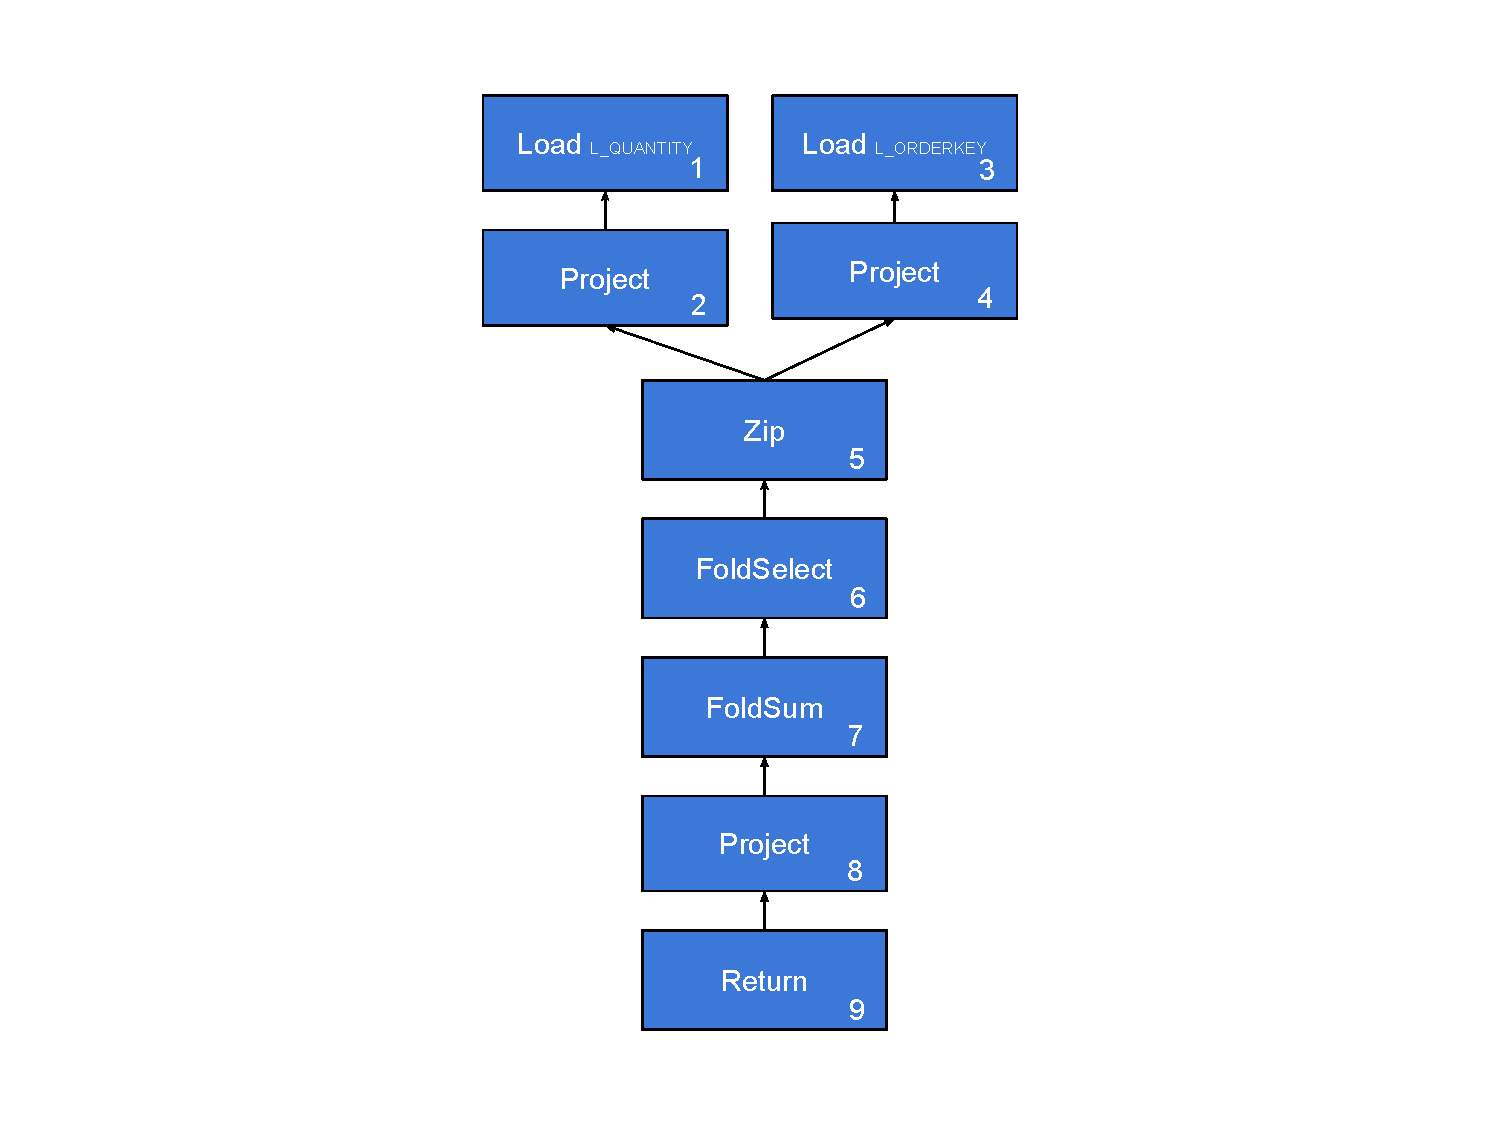
\includegraphics[width=\textwidth]{appendix/foldSelectQuery.pdf}
  \caption{A foldSelect Query which sums together all the quantities which have a non-zero order key}
  \label{fig:ASTfoldSelect}
\end{figure}%

\begin{figure}[h]
\centering
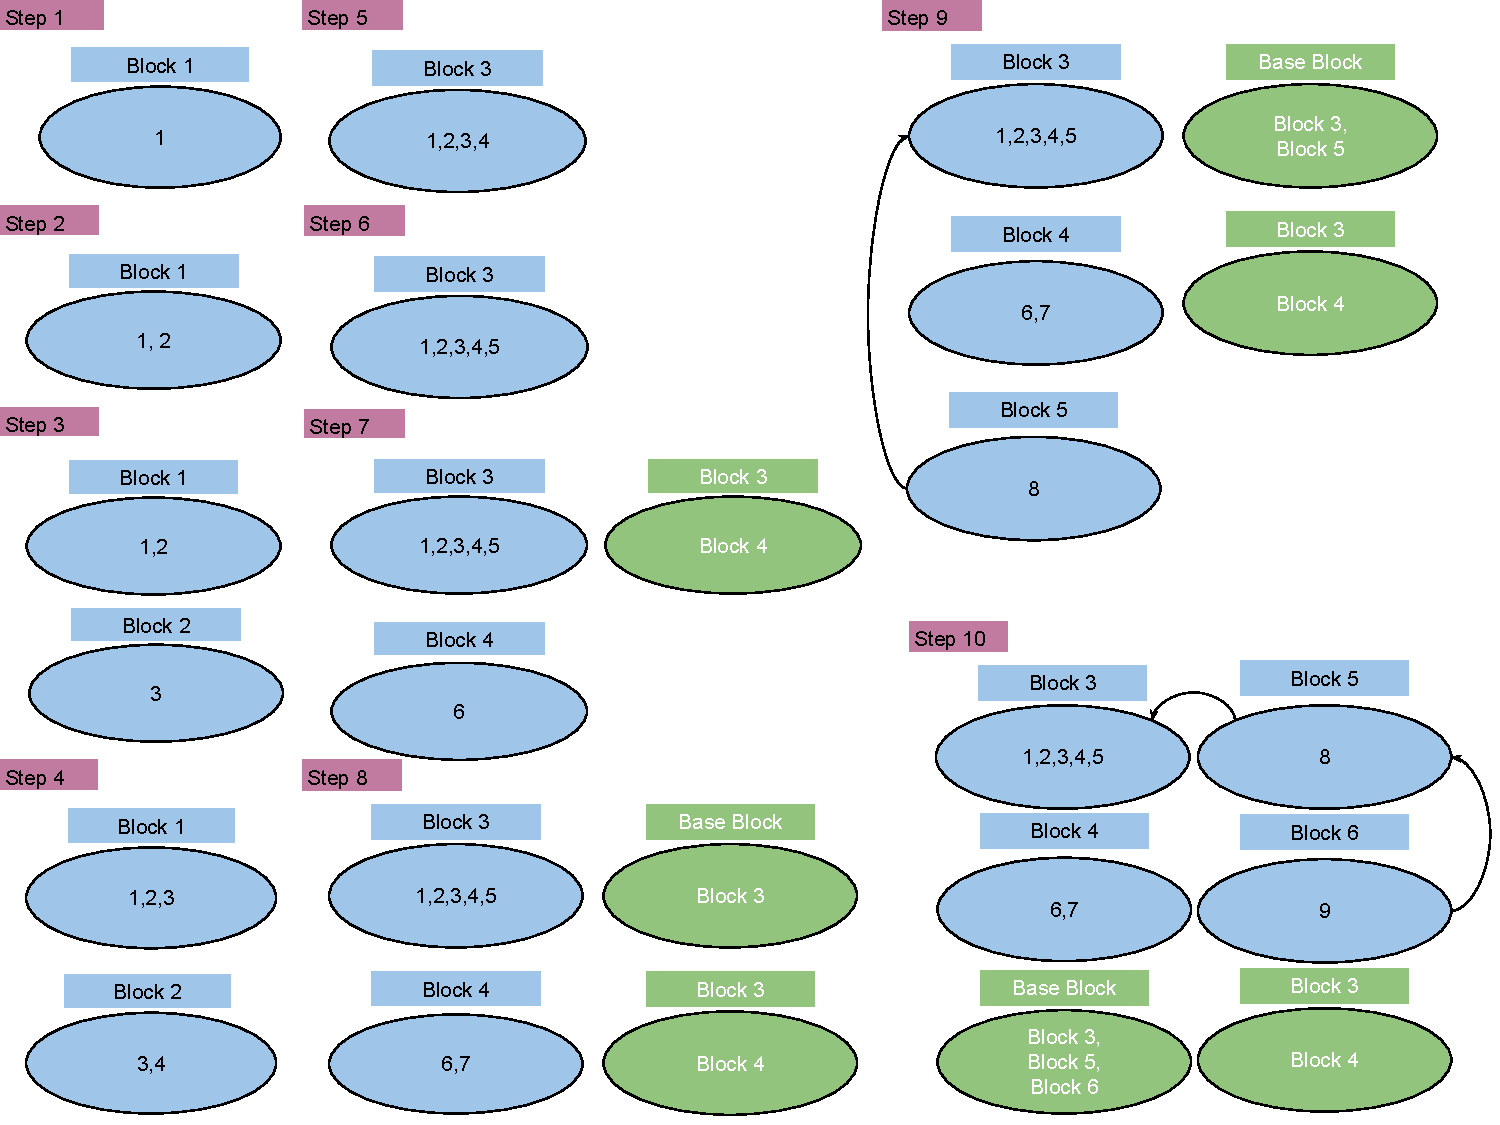
\includegraphics[width=1\linewidth]{appendix/FragmentConstructionFoldSelect.pdf}
\caption{Block Construction for a foldSelect Query. \ref{fig:ASTfoldSelect}}
\label{fig:fragmentConstructionfoldSelect}
\end{figure}

\begin{figure}
\begin{lstlisting}[frame=single, language=C]
__kernel void __runFragment0(
    __global int *persitent1, // L_QUANTITY column vector
    __global int *persitent3, // L_ORDERKEY column vector
    __global long *persistent10 // Result vector
) {
    struct {
        int fold;
        int value;
    } tmp5;
    int tmp6;
    int tmpAggregate7[32767] = {};
    int tmp8 = 0;
    for (int dominatingIteratorOffset = 0; 
         dominatingIteratorOffset < 3; 
         dominatingIteratorOffset += 1) {
        int tmp2 = persitent1[dominatingIteratorOffset];
        int tmp4 = persitent3[dominatingIteratorOffset];
        {
            tmp5.fold = tmp2;
            tmp5.value = tmp4;
        }
        {
            tmp6 = tmp5.value ? tmp5.fold : -1;
            if (tmp5.value) {
                tmp8 = tmpAggregate7[tmp6] = tmpAggregate7[tmp6] + tmp6;
            }
        }
    }
    int tmp9 = tmp8;
    persistent10[0] = tmp9;
}
\end{lstlisting}
    \caption{OpenCL code for \ref{fig:ASTfoldSelect}}
    \label{fig:openclCodeFoldSelect}
\end{figure}

\chapter{A Dynamic Programming Algorithm for Generating Blocks}
\label{appendix:dpalgo}
The current implementation of the block creation is a recursive algorithm. The problem of grouping statements together by the scope they belong to has an optimal substructure and there exists overlapping sub problems. An attempt has been made to convert the recursive solution into a dynamic programming solution.

Let us take the query represented in Figure \ref{fig:DPSimpleQuery}, specifically the \texttt{Zip} node. \texttt{Zip} operates on two vectors which in this case point to the same \texttt{Project} statement. The current implementation would recurse up the first vector and create a block and add the \texttt{Load} and \texttt{Project} statements. Once it has finished creating the block, it would recurse up the second vector that \texttt{Zip} depends upon, create a new block and add the same \texttt{Load} and \texttt{Project} call to that block. The algorithm would try and merge the blocks together and then proceed to add the \texttt{Zip} statement to the new merged block. This process is shown in figure \ref{fig:DPSimpleQueryFrag}.

An easy way to fix recursing over overlapping sub problems, is to use memoisation: have a map from the statement to the block it belongs in. If the statement already exists in a block, then return that block, instead of recreating it and merging it. This naive dynamic programming algorithm, has been implemented.

\begin{figure}
    \centering
    \begin{subfigure}{0.5\linewidth}
        \centering
        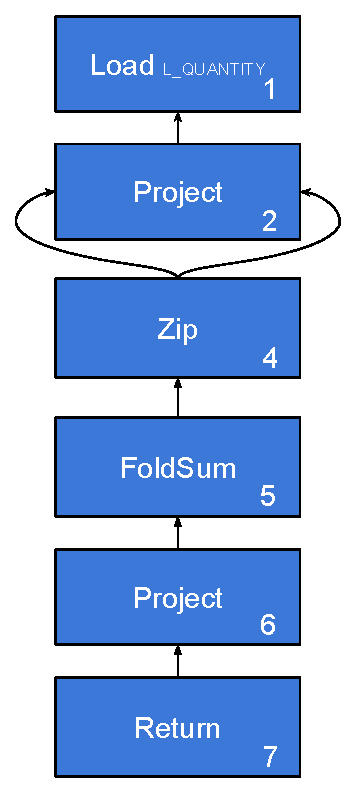
\includegraphics[width=0.5\linewidth]{appendix/DPExplain.pdf}
        \caption{An example query to show that there exists overlapping sub problems and has an optimal substructure}
        \label{fig:DPSimpleQuery}
    \end{subfigure}
    \begin{subfigure}{\linewidth}
        \centering
        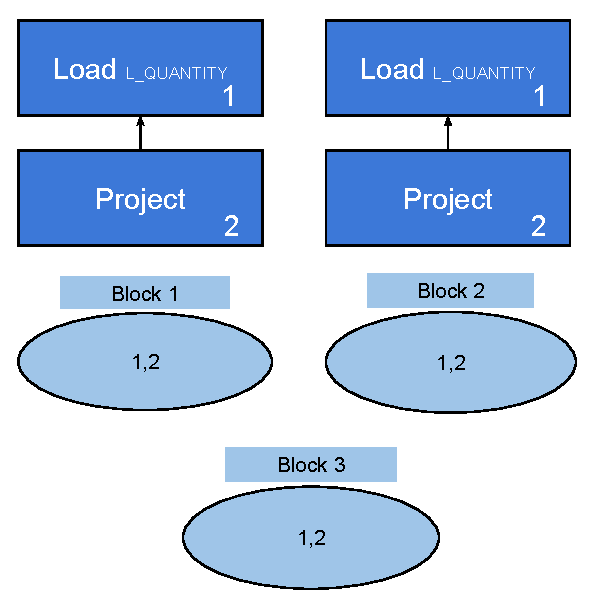
\includegraphics[width=0.5\linewidth]{appendix/DPExplainFrag.pdf}
        \caption{The process of creating blocks and merging blocks using the recursive solution before the zip statement can be added}
        \label{fig:DPSimpleQueryFrag}
    \end{subfigure}
    \caption{Caption}
    \label{fig:my_label}
\end{figure}

The case which our implemented naive dynamic programming algorithm does not handle, is the case presented in figure \ref{fig:dpedgeCase}. The figure shows what the final block creation looks like with the recursive algorithm. 


Using the naive dynamic programming algorithm, the algorithm would recurse up to the \texttt{Zip} statement. Then recurse up the first \texttt{requiredVector} and create the block (with block number 1) for the \texttt{Load}, \texttt{Project} and \texttt{FoldSum} statements. Once that block is created, the algorithm would recurse up the second \texttt{requiredVector} which in this case is a \texttt{Project} statement. As the \texttt{Project}'s \texttt{requiredVector} is a \texttt{Load} statement which already exists in block 1, it will return block 1 and add the \texttt{Project} statement to it. This is wrong! Instead of returning block 1, it should create a new block. This is because block 1 is reduced and the Zip statement depends on the result of the foldSum and therefore the zip statement and the block created from it's 2\textsuperscript{nd} \texttt{requiredVector} cannot belong with block 1 as it violates the 3rd condition to merge blocks. Figure \ref{fig:dpedgeCaseNaive} shows what the final block creation looks like with the naive dynamic programming algorithm. 

The block that will be created by the 2\textsuperscript{nd} \texttt{requiredVector} of the \texttt{Zip} statement is not aware about which blocks it can use to insert statements with or merge with. 

A possible solution is to pass a set of blocks that the 2\textsuperscript{nd} \texttt{requiredVector} cannot use and if a statement exists in the map, retrieve the block and check to see if that block is in the list banned blocks. If it is then create a new block instead of using the retrieved block.

Another possible solution, is to guarantee that unique load calls will be made for each set of statements that belong in the same scope. If this can be guaranteed, then the naive dynamic programming solution will work.

\begin{figure}
    \centering
    \begin{subfigure}{\textwidth}
        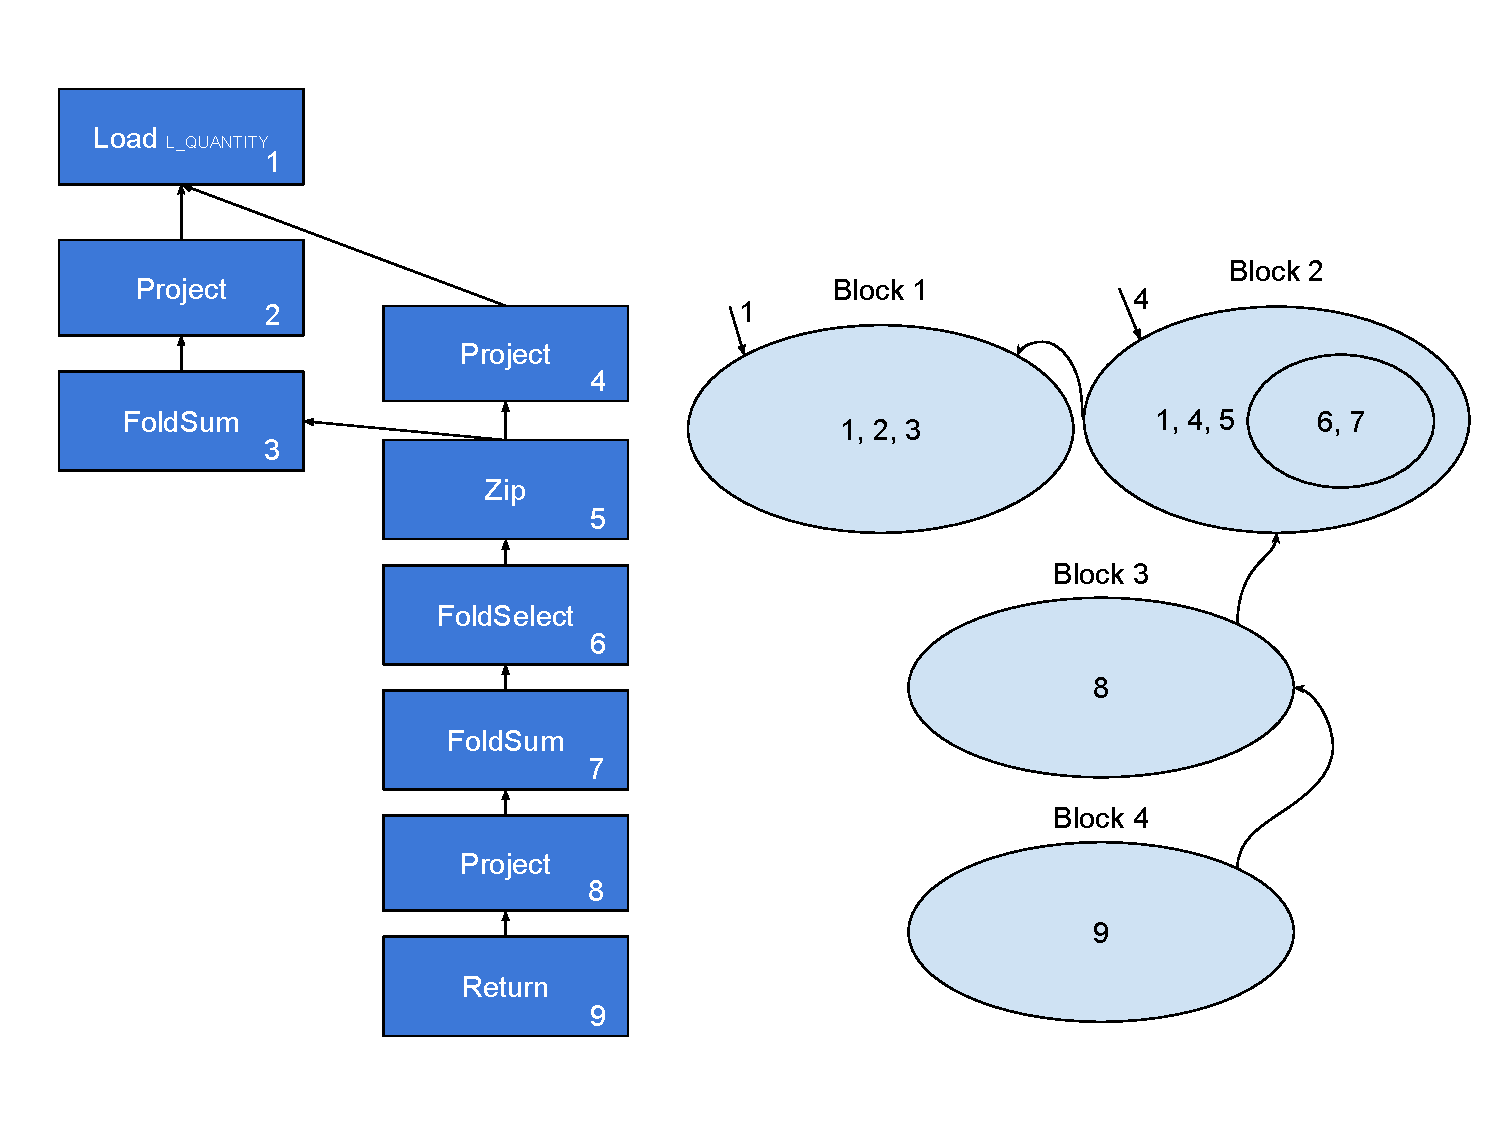
\includegraphics[width=\textwidth]{appendix/DPEdgeCase.pdf}
        \caption{An example query used to explain the edge case that is not handled by the naive dynamic programming algorithm. It also shows what the final stage of the blocks should look like using the recursive algorithm}
        \label{fig:dpedgeCase}
    \end{subfigure}
    \begin{subfigure}{0.6\textwidth}
        \centering
        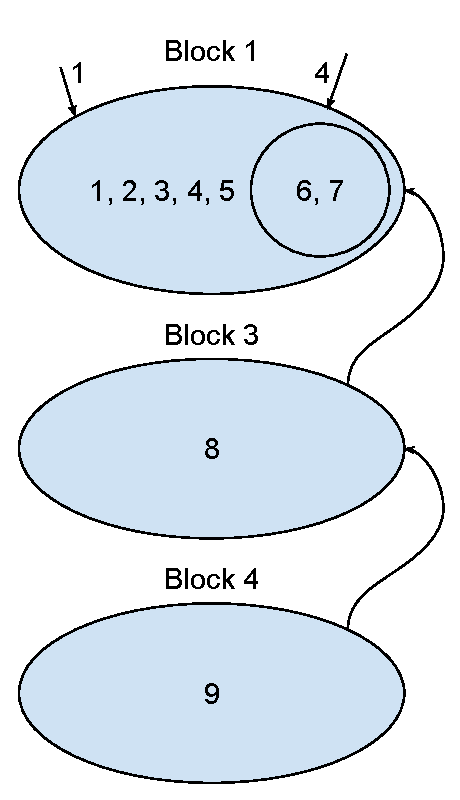
\includegraphics[width=0.5\linewidth]{appendix/DPNaive.pdf}
        \caption{Blocks created when the naive dynamic programming algorithm is used}
        \label{fig:dpedgeCaseNaive}
    \end{subfigure}
\end{figure}

\chapter{Metrics}
\label{appendix:metrics}

\section{Test Coverage}

\begin{figure}[H]
    \centering
    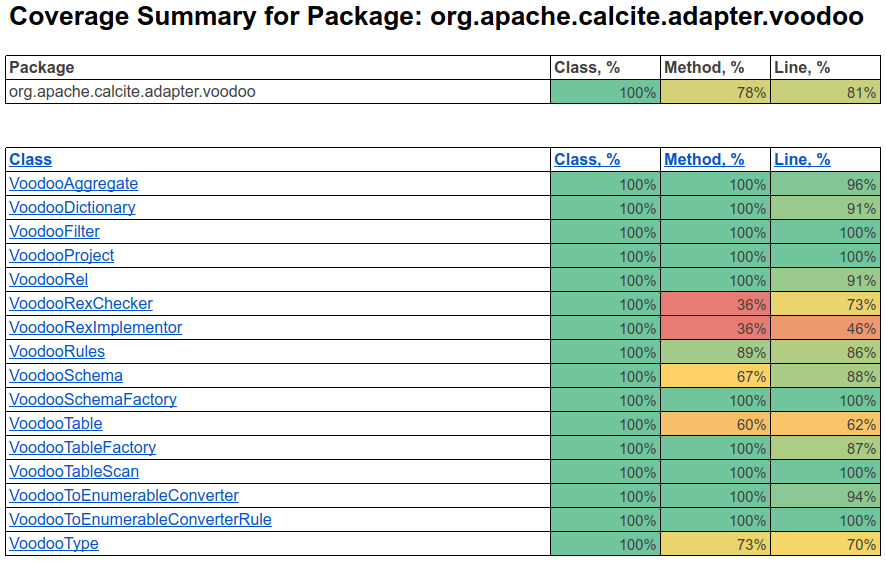
\includegraphics[width=0.7\linewidth]{evaluation/frontend-coverage.png}
    \caption{Font-end test coverage}
    \label{fig:fontend-cov}
\end{figure}

\begin{figure}[H]
    \centering
    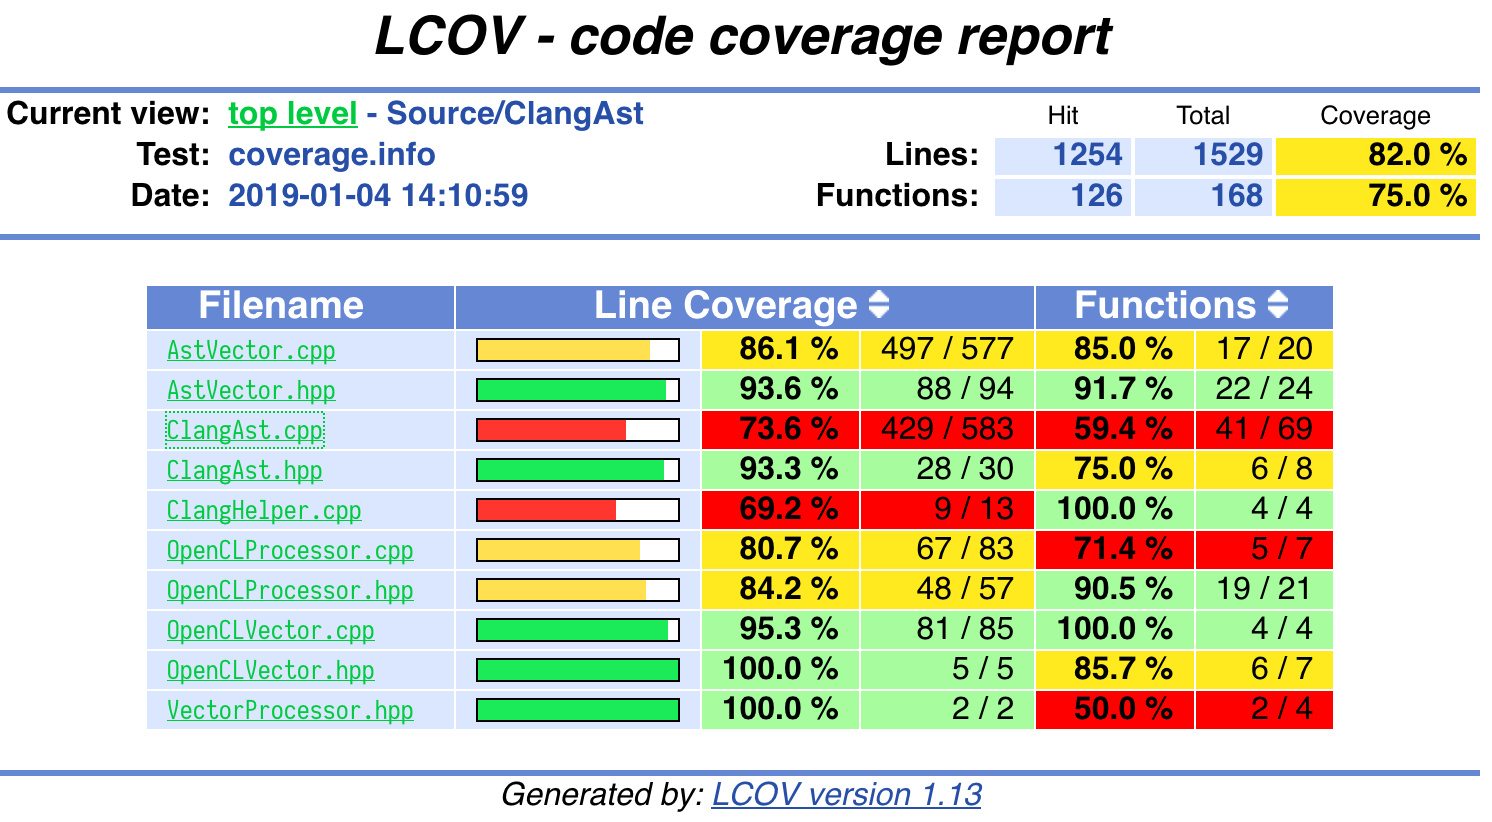
\includegraphics[width=0.75\linewidth]{evaluation/backend-coverage.png}
    \caption{Back-end test coverage.}
    \label{fig:backend-cov}
\end{figure}

\section{\texttt{Metrix++} results}

\begin{table}[H]
    \centering
    \begin{tabular}{@{}lllll@{}}
        \toprule
        \textbf{Metric}       & \textbf{Max} & \textbf{Avg} & \textbf{Total} \\ \midrule
        Cyclomatic Complexity & 71           & 1.29         & 1760           \\
        Maximum Indentation   & 11           & 1.41         & 1925           \\
        Magic Numbers         & 179          & 4.28         & 1341           \\ \bottomrule
    \end{tabular}
    \caption{\label{table:original-metrics}Original code results}
\end{table}

\begin{table}[H]
    \centering
    \begin{tabular}{@{}lllll@{}}
        \toprule
        \textbf{Metric}       & \textbf{Max} & \textbf{Avg} & \textbf{Total} \\ \midrule
        Cyclomatic Complexity & 71           & 1.86         & 820           \\
        Maximum Indentation   & 5            & 1.42         & 624            \\
        Magic Numbers         & 15           & 3.02         & 348           \\ \bottomrule
    \end{tabular}
    \caption{\label{table:opencl-metrics}\texttt{OpenCL} implementation results}
\end{table}

\begin{table}[H]
    \centering
    \begin{tabular}{@{}lllll@{}}
        \toprule
        \textbf{Metric}       & \textbf{Max} & \textbf{Avg} & \textbf{Total} \\ \midrule
        Cyclomatic Complexity & 24           & 1.05         & 128            \\
        Maximum Indentation   & 6            & 1.66         & 202           \\
        Magic Numbers         & 25           & 3.03         & 100           \\ \bottomrule
    \end{tabular}
    \caption{\label{table:clangast-metrics}\texttt{ClangAst} implementation results}
\end{table}

\paragraph{Disclaimer} These values should be taken with a pinch of salt. There are significant differences between the implemented algorithms, and different style choices were made.

Furthermore, the metric \emph{Magic Numbers} includes \textbf{0}s and \textbf{1}s and we do not know how \texttt{Metrix++} implements cyclomatic complexity.

\chapter{Dependencies}

\begin{table}[h]
    \centering
    \begin{tabular}{l l l}
        \hline
        \textbf{Repository} & \textbf{Dependency} & \textbf{License} \\
        \hline
        \texttt{calcite}    & Apache Calcite & Apache License 2.0 \\
        \texttt{calcite}    & Guava          & Apache License 2.0 \\
        \texttt{calcite}    & JUnit          & Eclipse Public License 1.0 \\
        \texttt{calcite}    & sqlline        & 3-Clause BSD License \\ 
        \hline
        \texttt{voodoo}     & Clang          & University of Illinois/NCSAOpen Source License \\
        \texttt{voodoo}     & OpenCL         & Khronos Specific License \\
        \texttt{voodoo}     & Boost          & Boost Software License \\
        \texttt{voodoo}     & Googletest     & 3-Clause BSD License \\
        \hline
        \texttt{voodoo-vis} & Axios          & MIT License \\
        \texttt{voodoo-vis} & Buefy          & MIT License \\
        \texttt{voodoo-vis} & Codemirror     & MIT License \\
        \texttt{voodoo-vis} & VisJS          & May be distributed under MIT or Apache 2.0 \\
        \texttt{voodoo-vis} & VueJS          & MIT License \\
        \hline
    \end{tabular}
    \caption{\label{table:dependencies}Licenses for each library used}
\end{table}

All software and packages detailed above are under licenses which would allow commercial use.

If this project was to be open-sourced, any copies of packages must include the original copyright texts and licenses (should we choose to distribute them along with our own source).

\end{document}